\documentclass{sig-alternate}

\usepackage{latexsym}
\usepackage{amsmath}
\usepackage{color}
\usepackage{graphicx}
\usepackage{amssymb}
\usepackage{epstopdf}
\usepackage{algorithmic}
\DeclareGraphicsRule{.tif}{png}{.png}{`convert #1 `dirname #1`/`basename #1 .tif`.png}



\def\punto{$\hspace*{\fill}\Box$}
\newcommand{\nop}[1]{}
\newcommand{\tuple}[1]{{\langle#1\rangle}}
\def\lBrack{\lbrack\!\lbrack}
\def\rBrack{\rbrack\!\rbrack}
\newcommand{\Bracks}[1]{\lBrack#1\rBrack}


\newtheorem{theorem}{Theorem}[section]
\newtheorem{proposition}[theorem]{Proposition}
\newtheorem{example}[theorem]{Example}
\newtheorem{remark}[theorem]{Remark}
\newtheorem{todo}[theorem]{ToDo}
\newtheorem{algorithm}[theorem]{Algorithm}

\nop{
\newtheorem{metatheorem}{Metatheorem}[section]
\newtheorem{definition}[theorem]{Definition}
\newtheorem{property}[theorem]{Property}
\newtheorem{corollary}[theorem]{Corollary}
\newtheorem{lemma}[theorem]{Lemma}
\newtheorem{conjecture}[theorem]{Conjecture}
\newtheorem{proviso}[theorem]{Proviso}
} % end nop




\conferenceinfo{SIGMOD}{'10 Indianapolis, IN}


%\title{The Cumulus System for Exact Online Aggregation in the Cloud}
%\title{Cumulus: A Distributed Exact Online Aggregation System}
%\title{Cumulus: Exact Online Aggregation by Message Passing}
\title{Exact Online Aggregation by Message Passing}


\numberofauthors{3}
\author{}%Oliver Kennedy, Yanif Ahmad, Christoph Koch}
\toappear{}


\begin{document}

\maketitle


\abstract{
We present Cumulus, a distributed exact online aggregation system.
Cumulus compiles a set of SQL aggregation queries
%
% or a datacube
%
down to a message-passing program that incrementally maintains
the query results by simple and highly efficient local modifications.
Surprisingly, for each tuple inserted, updated, or deleted,
our message passing programs
have to perform only a {\em constant}\/ amount of work per
aggregate value to be maintained.
%
%assuming constant-time read/write access to individual data items.
%This can be guaranteed if the data is kept in main memory.
%
Our message-passing protocol allows for massive parallelization.

The Cumulus runtime system is a distributed key-value store for
aggregate-group-by query results that implements our message passing protocol
for incremental result maintenance.
Cumulus efficiently answers OLAP queries using this store.
Cumulus performs the incremental maintenance of large views under
considerable update loads in realtime, leveraging parallelism
and using the resources of the cloud to keep its store in main memory.
}


\section{Introduction}


Recent years have seen the beginning of a paradigm shift in data management
research from incrementally
improving decades-old database technology
%
% (particularly, OLTP) -- System R and
% the long line of systems that have followed it --
%
to questioning established
architectures and creating fundamentally different, more lightweight systems
that are often domain-specific
(cf.\ e.g. \cite{DBLP:conf/vldb/StonebrakerMAHHH07,DBLP:journals/pvldb/KallmanKNPRZJMSZHA08}).
Part of the impetus for this change was given by 
potential users such as scientists and the builders of
large-scale Web sites and services such as Google, Amazon, and Ebay,
who have a need for data management systems but have found current databases
not to scale to their needs.
One can observe a trend to disregard database contributions
in these communities \cite{dbcolumn, DBLP:conf/sigmod/PavloPRADMS09}, and to build lightweight systems based on
robust technologies mostly pioneered by the operating systems and distributed
systems communities, such as large scale file systems, key-value stores, and
map-reduce
\cite{DBLP:journals/cacm/DeanG08, DBLP:journals/tocs/ChangDGHWBCFG08}.
Further impetus has resulted from the current need to develop data management
technology for multicore and cloud computing.
%
%, and by the example given by a
%number of innovative recent database startup companies that develop
%databases based on new architectures.
%\footnote{Examples are Vertica and Paraccel, who build column stores,
%and Greenplum, Asterdata, and Netezza, who take databases into the Cloud.}

There is a recent tendency among pundits outside the database community to
contest the need for powerful queries, and to
think of key-value stores -- with only the power to look up data by
keys -- as (much more efficient) database query engines.
%
%It shall not be denied that,
%with clever engineering, a surprising range of problems can be solved
%using key-value stores.
%
However, expressive query languages such as SQL do not cease to have
important applications and a substantial user base.
Alas, we do not know how to process SQL queries on updateable data
using a system as lightweight as a key-value store.

This paper contributes a fundamental and versatile building block for
enabling new, more lightweight and nimble data processing systems based
on SQL aggregation que\-ries. We believe that our contribution
constitutes an important
step towards achieving the contradiction in terms mentioned
above: executing complex aggregation queries on updateable data
using little more than a key-value store.

At the heart of our approach is a new aggressive recursive incremental
view maintenance mechanism.
In most traditional database query processors, the  basic building blocks of
queries are large-grained operators such as joins.
Our approach is based on compilation, reducing
queries to programs that are not based on classical query operators.
A large class of
SQL aggregation queries can be compiled down to very simple message
passing programs that incrementally maintain materialized views of
the queries. These message passing programs keep a hierarchy of map data
structures (which may be served out of a key-value store) up to date
and can share computation in the case that multiple aggregation queries (e.g.,
a data cube) need to be maintained.  Most importantly, though, these message
passing programs can be massively parallelized to the degree that the updating
of each single result aggregate value can be done in constant time on normal
off-the-shelf computers.\footnote{That is,
we assume that addition and multiplication
of {\em two numbers} can be performed in constant time, which is true for
%
%bounded precision numbers such as 
%
standard base types such as int and float,
but we assume no unrealistic models such
as aggregators with unbounded fan-in, as used in some theoretical models of
parallel computation. Our implementation indeed incrementally maintains
individual aggregate values in constant time. Note that since there are
usually many more aggregate values to maintain than there are processors,
this does not mean that each update is processed in constant time.
``Constant time'' is with respect to the size of the data, not the compiled
query.}
To the best of our knowledge, it was not known before
that this is possible.

In comparison, no such constant-time parallel processing technique
is known for nonincremental query
evaluation: Indeed, it is unlikely to exist.\footnote{Constant-time
bounded fan-in nonincremental
parallel processing is known not to be possible for
the class of queries we address,
unless the complexity class TC0 collapses into NC0, which it is not known
to do \cite{Joh90}.} Classical incremental view maintenance approaches, which
express the delta (=change) to a query result given an update again
as a (slightly simpler) query, fare no better: Generally,
given a query, there is another query whose delta is the first query.
Thus, classical incremental view maintenance has the same limits to
parallelization as nonincremental evaluation.


\subsection{Message passing programs}


We compile SQL aggregation queries to {\em map maintenance
message}\/ (M3) programs. An M3 program consists of a set of triggers of
the form
\[
\mbox{{\tt on insert into $R$($\vec{x}$) \{
($\vec{y}$:$D_{\vec{y}}$) $m[\vec{x}, \vec{y}]$ += $s$
\}}}
\]
or
\[
\mbox{{\tt on delete from $R$($\vec{x}$) \{
foreach $\vec{y}$ do $m[\vec{x}, \vec{y}]$ -= $s$
\}}}
\]
where $R$ is a relation name,
$\vec{x}$ and $\vec{y}$ are distinct tuples of variables and
$s$ is either a term or of the form
{\tt if $\phi$ then $t$ else 0}, where $t$ is a term.
Terms are built from addition, multiplication,
constants, variables from $\vec{x}$, external function calls $f(\vec{z})$,
and map accesses $m_1[\vec{z}_1], \dots, m_k[\vec{z}_k]$ where
$m$, $m_1$, $\dots$, $m_k$ are pairwise distinct
and the variables in $\vec{z}_1, \dots, \vec{z}_k$ are a nonoverlapping
subsets of the variables in $\vec{x}, \vec{y}$.
Conditions $\phi$ are conjunctions of comparisons $t'' \;\theta\; t'''$,
where $t'',t'''$ are terms without map accesses and
$\theta \in \{ =,<,\le,\neq \}$.
If $\vec{y}$ consists of zero variables, we omit
{\tt foreach $\vec{y}$ do}.
For each relation name, there may by multiple insert and delete triggers.

M3 programs can be read as straightforward pseudocode.
There are subtle issues to be discussed later about the domains of 
variable tuples
to be iterated over by foreach loops. Let us for now assume that
{\tt foreach $\vec{x}$ do $(\dots)$} iterates over all distinct tuples of
values currently in the
database, and that map values $m[\vec{x}]$ for $\vec{x}$ containing newly
inserted values are initially zero.


\begin{example}\em
\label{ex:TPCH-Q12}
Consider the following query on a TPC-H like schema,
which counts the number of LineItems per customer id.
\begin{verbatim}
SELECT   C.cid, SUM(1)
FROM     Customer C, Order O, LineItem L
WHERE    C.cid=O.cid AND O.oid=L.oid
GROUP BY C.cid;
\end{verbatim}
Here, cid is a key for the Customer relation and oid is a key for the
Order relation, but oid is not a key for LineItem.
Our compiler translates this query to the M3 program
\begin{verbatim}
on insert into Customer (cid, ...) { qO1[cid] += 1 }
on insert into Order (oid, cid, ...) {
  qL[cid, oid] += qO1[cid]
}
on insert into LineItem (oid, ...) {
  foreach cid do q[cid] += qL[cid, oid]
}
\end{verbatim}

In this and the following example, the delete-triggers are precisely
like the insert-triggers, but with {\tt +=} replaced by {\tt -=}.
Thus, to save space, the deletion triggers are omitted.

Let us ignore parallelization first.
It is not hard to see that this trigger program correct maintains the
query result, for each distinct {\tt cid} in Customer.cid, as {\tt q[cid]}.
(The maps {\tt qO1} and {\tt qL} are auxiliary.)
We assume that
there are no cascading deletes and, for instance, before we can delete an
Order, we have to delete all associated lineitems.
\punto
\end{example}


{\em Parallelization}.
The syntax of statements
\begin{equation}
\mbox{{\tt foreach $\vec{y}$ do $m[\vec{x}, \vec{y}]$ $\pm$= $s$}}
\label{eq:foreach}
\end{equation}
is misleading in that it suggests a loop --
that a nonconstant amount of work is needed to bring aggregate
values up to date. Of course, polynomial amounts of work are in fact need,
but only because in general there are many aggregate values -- in a
map representing the result of a group-by query or in an auxiliary map --
to be maintained. In fact, each statement of form (\ref{eq:foreach})
writes each value $m[\vec{x}, \vec{y}]$ only once and admits
{\em embarassing parallelism}: $m$ can be partitioned across many machines
that share the work.

Assume that the storage of individual maps
is partitioned across several machines. To execute a statement of form
(\ref{eq:foreach})
in a trigger invocation with arguments $\vec{x} = \vec{a}$,
where $s$ uses map lookups $m_i[\vec{x}_i, \vec{y}_i]$,
each node storing a value $m_i[\vec{a}_i, \vec{y}_i] = v$,
for $\vec{y}_i$ arbitrary, sends the message
$m_i[\vec{a}_i, \vec{y}_i] = v$ to the node managing value
$m[\vec{a}, \vec{y}]$. This way, that node receives all the values it
needs to update all $m$ values it represents.
Of course this requires a suitable protocol to ensure overall consistency
and that the right versions of map values are read and written in the right
order.



\begin{example}[star-join decomposition]\em
\label{ex:ssb}
Con\-sider \\ a simplified version of the star schema
benchmark (SSB) schema with relations Date(\underline{datekey}, year),
Part(\underline{partkey}, partcat), where partcat stands for a part category,
and LineOrder(datekey, partkey, revenue), which may contain duplicate tuples.
The query asks for the total revenues grouped by year and part category.

\begin{verbatim}
SELECT   P.partcat, D.year, SUM(revenue)
FROM     Date D, Part P, LineOrder L
WHERE    D.datekey=L.datekey
AND      P.partkey=L.partkey
GROUP BY P.partcat, D.year;

on insert into Date (datekey, year) {
  mPL[datekey, year] += 1
}
on insert into Part (partkey, partcat) {
  mDL[partkey, partcat] += 1
}
on insert into LineOrder (datekey, partkey, revenue) {
  foreach (partcat, year) do
  m[partcat, year] += revenue
                    * mDL[partkey, partcat]
                    * mPL[datekey, year]
}
\end{verbatim}

Observe how, on insertion into LineOrder, the code for incrementally
maintaining the query result {\tt m} decomposes into
two parts with disjoint variables, 
{\tt mDL[partkey, partcat]} and {\tt mPL[datekey, year]}.

The maps mPL and mDL have value at most
one at each position because datekey and partkey are keys for Date and Part,
respectively.

On insert into LineOrder, given values for
datekey and partkey, we instruct nodes
to send their {\tt mDL[partkey, x]} and {\tt mPL[datekey, y]} values,
for any {\tt x} and {\tt y},
to nodes maintaining {\tt m[x, *]} and {\tt m[*, y]}, respectively.
A node managing {\tt m[u, v]} receives, possibly from distinct nodes,
{\tt mDL[partkey, u]} and {\tt mPL[datekey, v]}
and can increment {\tt m[u, v]} by
{\tt revenue*mDL[partkey, u]*mPL[datekey, v]}.
%
%We only send nonzero {\tt mDL[partkey, x]} and {\tt mPL[datekey, y]} values,
%but at least an empty message so that the node managing m knows that it does
%not have to wait for anything more.
\punto
\end{example}


\begin{example}[self-join]\em
\label{ex:self-join}
We now ask, for each customer id (cid),
for the number of customers of the same nation (including the customer
identified by cid in the count).
\begin{verbatim}
SELECT   C1.cid, SUM(1)
FROM     Customer C1, Supplier C2
WHERE    C1.nation = C2.nation
GROUP BY C1.cid;
\end{verbatim}
The compiler produces the following on-insert trigger:
\begin{verbatim}
on insert into Customer (cid, nation) {
  q[cid] += qC1[nation];
  foreach cid2 do q[cid2] += qC2[cid2, nation];
  q[cid] += 1;
  qC1[nation] += 1;
  qC2[cid, nation] += 1
}
\end{verbatim}
The on-delete trigger is just like the on-insert trigger with {\tt +=}
changed to {\tt -=} everywhere other than in the third statement
({\tt q[cid] += 1}), which remains unchanged.
We will establish later that this M3 program is indeed correct.

For now, we challenge the reader to find a 
fundamentally different (ideally, simpler) way to
perform the incremental maintenance of {\tt q}
which has the M3 property of embarassing parallelism, with each value
to be updated only requiring a constant amount of work.
Examples~\ref{ex:TPCH-Q12} and \ref{ex:ssb} were chosen for simplicity,
but we believe that this example shows that creating M3 programs in general
is nontrivial.
\punto
\end{example}


It shall be emphasized that for each of the examples of this section,
and the paper as a whole, our compilation approach produces exactly
the M3 programs shown.


The fragment of SQL queries that we can compile to M3 essentially comprises
SUM-agg\-regation queries with group-by.
COUNT and AVG queries can be defined by arithmetic expressions over these.
We exclude MIN and MAX queries, aggregation
nested into FROM or WHERE clauses, the DISTINCT and HAVING keywords,
outerjoins,
and the relational difference operation. At the end of this paper, we will
discuss which of these features can be added without fundamental difficulties.


\subsection{The Cumulus System}


We have developed a system, Cumulus\footnote{A Cumulus cloud is an
aggregation cloud, thus the name.}, that parallelizes the
execution of M3 programs in a cluster or computing cloud.
Cumulus performs incremental maintenance of exact aggregation views online, and
executes an efficient
protocol to ensure consistency of map data and query results,

While it is no fundamental requirement of our compilation
approach, we have chosen to use the resources of the cloud to maintain
the data in main memory, allowing for very low latency updating and querying.
At the time of writing this,
Terabyte-sized memory chips (DIMMs and flash) have already been announced by
manufacturers, and already now, large data warehouses
can be run in main memory in the cloud, where additional hardware costs
(main memory is more expensive per TB than hard disks) are
offset by greater robustness of the system, lower maintenance
costs, lower heat production \cite{1154557}, and of course by of orders
of magnitude better speed and latency characteristics.

The Cumulus protoype aims at demonstrating our results in the context of
pushing OLAP into the cloud.
Cumulus automates  the process of  creating, loading,
and  maintaining  in-memory  data  warehouses.
(Optional logging of updates to secondary storage
for persistency is supported.)
Cumulus targets OLAP applications  that perform real-time analytics of
relational data.  By feeding it an SQL query, Cumulus's infrastructure
becomes linked to  a set of OLTP databases.  Cumulus  keeps the
data warehouse synchronized with the source databases via an
update stream. It achieves synchronization {\em in realtime}
through parallelization, keeping data in main memory, and our approach of
query processing by message passing.


\subsection{Contributions and Structure of the Paper}


Our main technical contributions are as follows.
\begin{itemize}
\item
We present M3, a massively parallelizable language
for message passing programs that can be used to incrementally maintain
SQL aggregation queries.

\item
We describe our compiler for translating SQL aggregation queries to M3
programs. Our compilation technique is based on a novel, aggressive, recursive
form of incremental view maintenance.

\item
We present Cumulus, our system for exact online aggregation in realtime.
We describe the Cumulus message passing protocol, which assures
consistency of the maps using only few messages, and
infrastructure, and show how it can be used to efficiently distribute the
processing and storage requirements of query processing and
the incremental maintenance of large aggregate views and datacubes.

\item We show evidence for the scalability of our approach by examining the
performance of Cumulus on examples drawn from the TPC-H\cite{tpch2008}
benchmark. 
\end{itemize}


The remainder of this paper is organized as follows.
Section \ref{sec:compiler} describes our SQL to M3 compiler.
In Section \ref{sec:architecture}, we provide an overview of Cumulus's online
infrastructure and discuss how data is managed within that infrastructure.
Section \ref{sec:experiments} presents
experimental results that demonstrate the viability and scalability of
Cumulus.
Section \ref{sec:relatedwork} discusses related work.
The paper concludes with Section \ref{sec:conclusions}







\section{Compilation to M3}
\label{sec:compiler}


\subsection{Query Calculus}


\def\safe{\mbox{safe}}
\def\AggSum{\mbox{Sum}}

Our calculus consists of
{\em formulae} of positive quantifier-free relational domain calculus
(i.e., formulae constructed from conjunctions ``and'',
disjunctions ``or'', and atoms) and of {\em terms}.
%
The atomic formulae are {\em true}, {\em false}, relational atoms $R(\vec{x})$
where $\vec{x}$ is a tuple of variables,
and atomic constraints of the form $t_1 \;\theta\; t_2$ comparing two terms
$t_1$ and $t_2$ using comparison operations $\theta$ of $=$, $\neq$, $<$,
and $\leq$.
%
Terms are built from variables, constants, built-in function calls
$f(\vec{t})$, where $\vec{t}$ is a tuple of terms,
and aggregrate sums ($\AggSum$) using addition and multiplication.
Built-in functions compute their result entirely based on their input
terms, not accessing the database (e.g., mod or string concatenation).
In short, the grammar for formulae $\phi$ and terms $t$
(given variables $x$, constants $c$, relation names $R$,
comparison operators $\theta$,
and builtin functions $f$) is
\begin{eqnarray*}
  \phi &\mbox{::-}& \phi \land \phi
               \mid \phi \lor \phi \mid (\phi)
               \mid \mbox{true} \mid \mbox{false} \mid R([x(,x)^*])
               \mid t \;\theta\; t
\\
  t &\mbox{::-}& t * t \mid t + t \mid (t) \mid c \mid x \mid f([t(,t)^*]) \mid
                 \AggSum(t, \phi)
\end{eqnarray*}

An aggregate term $\AggSum(t, \phi)$
is {\em constraints-only} if $\phi$ does not
contain relational atoms $R(\vec{x})$ (but atomic constraints $s \theta t$).
We can also think of such an aggregate term as a (functional)
if-statement (if $\phi$ then t else 0)
or, using C syntax, ($\phi$ ? $t$ : 0).

We will make one important syntactic restriction, namely that
no $\AggSum$ terms may occur in atomic constraints.

Formulas and terms are evaluated relative to a given set of
{\em bound variables}.
The bound variables of a subformula are the bound variables of the formula.

Given a set of bound variables $B$,
the {\em safe variables} of a formula are defined bottom-up
as usual in relational
calculus (see e.g. \cite{DBLP:books/aw/AbiteboulHV95}). In particular,
\begin{eqnarray*}
\safe_B(R(\vec{x})) &:=& \{x_i\} \cup B \\
\safe_B(\phi \land \psi) &:=& \safe_B(\phi) \cup \safe_B(\psi) \\
\safe_B(\phi \lor \psi)  &:=& \safe_B(\phi) \cap \safe_B(\psi) \\
\safe_B(\phi \land x = y) &:=&
\left\{\begin{array}{ll}
\safe_B(\phi) \cup \{ x, y \} &\dots
\mbox{$x$ or $y$ is} \\
&\;\;\; \mbox{in $\safe_B(\phi)$} \\[.5ex]
\safe_B(\phi) &\dots \mbox{otherwise}.
\end{array} \right.
\end{eqnarray*}
Here $\{x_i\}$ drops order and turns the tuple $\vec{x}$ into a set.

Given a term $\AggSum(t, \phi)$ with bound variables $B$,
the bound variables of $\phi$ are $B$ and the bound variables of $t$ are
the safe variables of $\phi$, $\safe_B(\phi)$.
The bound variables of a subterm are the bound variables of the term.
Variables occuring as terms must be bound.

\begin{example}\em
Given singleton bound variable set $\{ y \}$,
\[ \AggSum(u * f(z), \underbrace{(\underbrace{(\underbrace{R(x, z)}_{x,y,z} \lor \underbrace{y=z}_{y,z})}_{y,z} \land z = w)}_{y,z,w}) \]
is invalid: The safe variables of the formula are
$\{y,z,w\}$, so $u$ is not bound in the term $u * f(z)$. The overall term
becomes valid for bound variables $\{u,y\}$.
\punto
\end{example}


\def\db{{\cal{A}}}

The semantics of formulas and terms is given by a (polymorphic) function
$\Bracks{\cdot}(\cdot, \cdot)$ that takes a database and values for the
bound variables as arguments. Given database $\db$ and values $\vec{b}$ for
the bound variables,
$\Bracks{\phi}(\db, \vec{b})$ evaluates to a relation and
$\Bracks{t}(\db, \vec{b})$ evaluates to a value of the type of
terms.\footnote{In practice,
we have several types such as integers and floats, but
here we will not talk about types and will assume that all terms evaluate to,
say, floating point numbers. However, our implementation supports the
main data types of SQL, and no noteworthy observations were made achieving
this.}
We assume a multiset semantics for relations, which is important to note
since we focus on computing aggregates. The multiset semantics of formulas
is defined by their well-known translation to relational algebra
(Codd's theorem), and the standard multi-set semantics of
(in our case, positive) relational algebra. 
$\AggSum$ terms are new, but otherwise the
semantics of terms is obvious.
A term $\AggSum(t, \phi)$
computes the sum of the values $t[\vec{x}]$
over the distinct valuations (with duplicates)
of the safe variables $\vec{x}$ of $\phi$, i.e.,
given a database $\db$ and values $\vec{b}$ for the bound variables of $\phi$,
\[
\Bracks{\AggSum(t, \phi)}(\db, \vec{b}) =
\sum_{\vec{v} \;\mathrm{in}\; \Bracks{\phi}(\db, \vec{b})} \Bracks{t}(\db, \vec{v}).
\]


{\bf From SQL to the Calculus}.
Given our semantics definition, the translation from SQL to our calculus is
straightforward.
%
%We focus on aggregation queries, specifically
%sum aggregation queries (count and avg aggregation queries can be encoded
%using sum). Aggregates can be nested in the SELECT clause, but not in
%the FROM, WHERE, or HAVING clause. We support GROUP by, although in a way
%that may at first seem nonstandard. We do not support DISTINCT.
%
A SQL aggregate query
\begin{verbatim}
SELECT groupcols, SUM(t)
FROM   R1 r11, R1 r12, ..., R2 r21, ...
WHERE  cond
GROUP BY groupcols
\end{verbatim}
is expressed in the calculus as
\[
\AggSum(t, R_1(\vec{x}_{11}) \land R_1(\vec{x}_{12}) \land \dots
\land R_2(\vec{x}_{21}) \land \dots \land \mbox{cond})
\]
with {\em bound variables} groupcols.


\begin{example}\em
\label{ex:self-join-calc}
The query of Example~\ref{ex:self-join} translates to
$\AggSum(1, \mbox{Customer}(c_1,n_1) \land \mbox{Customer}(c_2, n_2) \land
n_1=n_2)$ in the calculus, with bound variable $c_1$.
\punto
\end{example}

\subsection{Normalization and Simplification}


A semiring is an algebra with two associative operations,
$+$ and $*$, that
have neutral elements (called 0 and 1, respectively), which satisfy
distributivity ($a*(b+c)= a*b + a*c$), and where $+$ is commutative.
Semirings with variables
have polynomials, that is, each expression of the
semiring can be mapped to an equivalent expression that is
a sum of flat products (the products are also known as {\em monomials}\/).
Turning semiring expressions into polynomials just means to apply
distributivity repeatedly until we end up with a polynomial.
This can be combined with simplification operations based on the 1 and
0-elements, i.e., $\alpha * 1$ maps to $\alpha$, $\alpha*0$ maps to $0$, and
$\alpha+0$ maps to $\alpha$. Polynomials can be conveniently implemented
as lists of lists of atoms, where an empty top-level list (i.e., polynomial)
has value 0 and an empty monomial list has value 1.

Both our formulae and our terms are semirings; in particular,
in the semiring of formulae, $\land$ is the product operation,
$\lor$ is addition,
and $\textit{false}$ and $\textit{true}$ are 0 and 1, respectively.

For arbitrary terms $s$ and $t$ and formulas $\phi$ and $\psi$,
$\AggSum$ terms can be simplified using the following equations (to be
applied by replacing a left by a right hand side expression)
\begin{eqnarray*}
\AggSum(t, \textit{true}) &=& t \\
\AggSum(t, \textit{false}) &=& 0 \\
\AggSum(0, \phi) &=& 0 \\
\AggSum(s+t, \phi) &=& \AggSum(s, \phi) + \AggSum(t, \phi) \\
\AggSum(t, \phi \lor \psi) &=& \AggSum(t, \phi) + \AggSum(t, \psi)
\end{eqnarray*}

All these algebraic laws can be applied, and the calculus expression
be maximally simplified, in a single bottom-up pass of the expression.
A term ($\AggSum$ or other) maximally simplified in this way
is a sum of terms that contain neither $+$ nor $\lor$; we call such 
normalized terms {\em recursively monomial}.
Define function RecMonomials to compute the list of recursively monomials
of a term.

\def\vars{\mbox{vars}}

{\bf Factorization of monomial aggregate terms}.
For $e$ either a formula or a term, let $\vars(e)$
be the set of all variables occurring in $e$.
Factorization employs the equivalence
\[
\AggSum(s*t, \phi \land \psi) = \AggSum(s, \phi) * \AggSum(t, \psi)
\]
which is true if
$(\vars(s) \cup \vars(\phi)) \cap (\vars(t) \cup \vars(\psi)) = \emptyset$.

Consider an aggregate term $\AggSum(t, \phi)$ where both $t$ and $\phi$ are
monomials, consisting of the sets $T$ and $F$ of atomic terms and formulae,
respectively (that is, $t = \prod T$ and $\phi = \bigwedge F$).
We can think of the
elements of the two-sorted set $T \cup F$ as the hyperedges of a
{\em hypergraph},
where the function $\vars(e)$ maps hyperedge $e$ to the nodes that are
part of it.
The set of {\em connected components} ${\cal C}$ of this hypergraph is the
maximum cardinality set of subsets of $T \cup F$ such that for any
two components $C_1, C_2 \in {\cal C}$ with $C_1 \neq C_2$,
$\vars(C_1) \cap \vars(C_2) = \emptyset$. Asking for the maximum number of
nonoverlapping components is of course the same as asking for components of
minimum size, and the set of connected components is unique and can be computed
in linear time using Tarjan's algorithm. Given ${\cal C}$, each component
$C \in {\cal C}$ can again be partitioned by sort into a monomial term $t_C$
and a monomial formula $\phi_C$.
%
% By convention, if $C$ does not contain atomic terms, $t_C = 1$ and if $C$
% does not contain atomic formulae, $\phi_C = \textit{true}$. It is not
% difficult to verify that
%
$\AggSum(t, \phi)$ is equivalent to
\[
\prod_{C \in {\cal C}} \AggSum(t_C, \phi_C).
\]

{\em Recursive factorization}, given term $\AggSum(t, \phi)$, first recursively
factorizes the aggregate terms in $t$ before applying factorization as
just described on the top level.


\begin{example}\em
The connected components of term
\[
\AggSum(5 * x * \AggSum(1, R(y, z)) * w, R(x,y) \land S(z) \land R(v, w))
\]
are
$\{ \{5\}, \{ x, R(x,y), \AggSum(1, R(y, z)), S(z) \}$,
$\{ w, R(v, w)) \} \}$
and thus the term factorizes as
$\AggSum(5, \textit{true}) *
\AggSum(x * \AggSum(1$, $R(y, z)), R(x, y) \land S(z)) *
\AggSum(w, R(v, w)))$.
$\AggSum(5, \textit{true})$ simplifies to $5$.
\punto
\end{example}


{\bf Variable elimination}.
Given an abitrary monomial formula $\phi = \bigwedge (E, O)$,
where $E$ are the equality
atoms $x=y$ and $O$ are the remaining atoms (either set may be empty) and
a set of bound variables $B$.
We eliminate redundant variables as follows.

Consider the equivalence classes of the equivalence relation $E$.
For each equivalence class $C$ of $E$, distinguish an element
(i.e., variable) as $x_C$ such that,
if $B \cap C \neq \emptyset$, $x_C$ is an arbitrary element of $B \cap C$;
otherwise, it is an arbitrary element of $C$.
Create a unification mapping
$\Theta$ that maps each unbound variable $y$ of $E$ to $x_{[y]}$ (where $[y]$ is the
equivalence class of $y$) and is the identity on the bound variables.
Now substitute all variables in $O$
using $\Theta$, obtaining $O'$. Let
$E' =  \bigcup \{ y = x_{[y]} | y \in ((B \cap [y]) -  x_{[y]}) \}$.
Then we replace $\phi$ by $(\bigwedge O') \land \bigwedge E'$.

Given a term $\AggSum(t,\phi)$ where $\phi$ is a monomial,
and bound variables, we eliminate variables by 
first eliminating variables in $\phi$, creating $\phi'$ and $\Theta$.
Then we substitute all variables of $t$ that are in the domain of $\Theta$
using $\Theta$, obtaining $t'$. The result, $\AggSum(t', \phi')$, is equivalent
to $\AggSum(t,\phi)$.


\begin{example} \em
Given term $\AggSum(y*v*r, R(z, v) \land v<q
\land x=y \land x=z \land u=v \land v=w \land q=r)$
and bound variables $\{x,y,z,r\}$.
The variable equivalence classes are
$\{ \{x,y,z\}, \{u,v,w\}, \{q,r\} \}$. We chose the rightmost variable in
each class as the variable to substitute by. In the first class, we can choose
freely because all members are bound. In the second we can choose freely
because none are bound. In the third, we must choose $r$ because it is bound
and $q$ is not.
The mapping is
$\Theta = \{ x \mapsto x, y \mapsto y, z \mapsto z, u \mapsto w, v \mapsto w,
w \mapsto w, q \mapsto r, r \mapsto r \}$.
We apply $\Theta$ to $y*v*r$ and $R(z, v) \land v < q$ and obtain
$z*w*r$ and $R(z,w) \land w<r$, respectively. The simplified
overall term is
$\AggSum(z*w*r, R(z,w) \land w<r \land x=z \land y=z)$.
\punto
\end{example}


{\bf Extraction of aggregates}.
For a term $t$ and its set $B$ of bound variables,
the function ExtractAggregates($t$, $B$)
replaces each maximal subterm $s$ of $t$
that is of the form $\AggSum(\cdot, \cdot)$ but is not constraints-only
by a ``map access''  $m[\vec{x}]$, where
$m$ is a new name and $\vec{x}$ is the set of variables
both bound at $s$ and used in $s$ ordered arbitrarily.
The result of ExtractAggregates thus is a pair $(t', \Theta)$ of the remainder
term $t'$ and a mapping $\Theta$ from map accesses $m[\vec{x}]$ to extracted
subterms $s$ (which could be used to undo the extraction).

\begin{example}\em
Let $t$ be the term
\begin{multline*}
\AggSum(x*\AggSum(w, R(v, w), R(w, z)), x<y \land y=z) \\
*\; 5 * y * \AggSum(u, R(u, x)).
\end{multline*}
Then ExtractAggregates($t$, $\{x,y\}$) returns the pair consisting of term
$\AggSum(x*m_1[z], x<y \land y=z) * 5 * y * m_2[x]$
and the mapping
$\{
m_1[z] \mapsto \AggSum(w, R(v, w), R(w, z));
m_2[x] \mapsto \AggSum(u, R(u, x))
\}$.
\punto
\end{example}


{\bf Lifting ifs}. Observe that if $\phi$ is a constraints-only term in which
all variables are bound, then
\begin{eqnarray*}
\AggSum(t, \phi \land \psi) &=& \AggSum(\AggSum(t, \psi), \phi) \\
t * \AggSum(t', \phi) &=& \AggSum(t * t', \phi)
\end{eqnarray*}
Thus we can lift $\phi$ to the top of a recursively monomial term.
Let function LiftIfs do exactly this.

\begin{example}\em
This will be used in Example~\ref{ex:self-join-compile}:
\begin{multline*}
\mbox{LiftIfs}((-1) * \AggSum(1, C(c_2, n) \land c_1=c), \{c_1, c, n\}) = \\
\AggSum((-1) * \AggSum(1, C(c_2, n)), c_1=c).
\end{multline*}
\end{example}


Given a recursively monomial term $t$ and a set of bound variables $B$,
let the function Simplify($t$, $B$) recursively factorize $t$, then perform
variable elimination, and finally if-lifting.


\subsection{Delta Computation}


\def\dt{\Delta_{\pm R(\vec{t})}}


Given a term or formula $\alpha$
of our calculus, and an insertion or deletion of a
single tuple $\vec{t}$ to/from a relation $R$ of the database.
We denote the database obtained from database $\db$ by this update by
$\db \pm R(\vec{t})$.
We can express a delta $\Delta_{\pm R(\vec{t})} \alpha$
(which is a term if $\alpha$ is a term and a formula if $\alpha$ is a formula)
such that,
given current database $\db$ and values $\vec{b}$ for the bound variables,
\begin{eqnarray}
\Bracks{\alpha}(\db \pm R(\vec{t}), \vec{b}) &=&
\,\Bracks{\alpha}(\db, \vec{b}) \pm \,\Bracks{\dt \alpha}(\db, \vec{b}).
\label{eq:delta}
\end{eqnarray}

The delta rules for semirings are as follows. We use $+$ and $*$ for the
addition and multiplication operations; for formulae, these are of course
$\lor$ and $\land$, respectively.
\[\begin{array}{lllcr}
\dt (\alpha + \beta) &:=& ((\dt \alpha)    &+& (\dt \beta))
\\[1ex]
\dt (\alpha \,*\, \beta)
   &:=& ((\dt \alpha)               &*& \beta\;\,) \\
   &+ & (\quad\quad\quad\;\, \alpha &*& (\dt \beta)) \\
   &+ & ((\dt \alpha)               &*& (\dt \beta))
\end{array}\]

For atomic formulae and terms,
\[\begin{array}{lllr}
\dt \AggSum(t, \phi)
   &:=& \AggSum((\dt t), & \phi\;\,) \\
   &+ & \AggSum(\quad\quad\quad\; \,t,  & (\dt \phi)) \\
   &+ & \AggSum((\dt t), & (\dt \phi))
\\[1ex]
\dt R(x_1, \dots, x_k) &:=& \big( \bigwedge_{i=1}^k (x_i = t_i) \big)^\pm
\end{array}\]
and, for $S$ a relation different from $R$,
\[
\dt S(x_1, \dots, x_l) := \textit{false}.
\]
For all other atomic terms and formulae, $\dt$ is the zero-element
of their respective semirings (that is, $0$ and $\textit{false}$,
respectively.)

Here $(\cdot)^\pm$ is an annotation that we do not give a formal semantics
to for space limitations, but explain how to eliminate. $\phi^+$ is just
$\phi$ and $\phi^-$ intuitively defines a relation of ``negative'' tuples.
We define $\phi^- \land \psi = \phi \land \psi^- = (\phi \land \psi)^-$,
$\phi^- \land \psi^- = \phi \land \psi$, and
$\AggSum(t, \phi^-) = -\AggSum(t, \phi)$. To
push $(.)^-$ up beyond $\lor$, we first compute
a DNF, push $\lor$ out of the formula across $\AggSum$, and then apply
the above rules to the remaining monomial formulae.
For example,
$\AggSum(t, \phi \land (\psi \lor \pi^-)) =$
$\AggSum(t, \phi \land \psi) + \AggSum(t, \phi \land \pi^-) =$
$\AggSum(t, \phi \land \psi) - \AggSum(t, \phi \land \pi)$.


\begin{proposition}
\label{prop:delta-correct}
This definition of $\dt$ satisfies Equation \ref{eq:delta}.
\end{proposition}


\def\duv{\Delta_{\pm R(u,v)}}
\def\dc{\Delta_{\pm C(c,n)}}


\begin{example}\em
\label{ex:self-join-delta}
Consider the query of Example~\ref{ex:self-join}, which translates to the
calculus as
\[
q[c_1] = \AggSum(1, C(c_1,n_1) \land C(c_2, n_2) \land n_1=n_2)
\]
where $C$ is short for Customer (see Example~\ref{ex:self-join-calc}).
Now, since $(\dc n_1=n_2) = 0$ and thus
\[
(\dc C(c_2, n_2) \land n_1=n_2) = (c_2=c \land n_2=n)^\pm \land n_1=n_2,
\]
\begin{multline*}
\dc \AggSum(1, C(c_1,n_1) \land C(c_2, n_2) \land n_1=n_2) = \\
\AggSum(1, \dc (C(c_1,n_1) \land (C(c_2, n_2) \land n_1=n_2))) = \\
\AggSum(1, 
((c_1=c \land n_1=n)^\pm \land (C(c_2, n_2) \land n_1=n_2)) \lor \\
(C(c_1,n_1) \land (c_2=c \land n_2=n)^\pm \land n_1=n_2) \lor \\
((c_1=c \land n_1=n)^\pm \land (c_2=c \land n_2=n)^\pm \land n_1=n_2) =
\end{multline*}

\vspace{-6mm}

\begin{eqnarray*}
&\pm& \AggSum(1, c_1=c \land n_1=n \land C(c_2, n_2)       \land n_1=n_2) \\
&\pm& \AggSum(1, C(c_1,n_1)        \land c_2=c \land n_2=n \land n_1=n_2) \\
&+&   \AggSum(1, c_1=c \land n_1=n \land c_2=c \land n_2=n \land n_1=n_2)
\end{eqnarray*}

Simplifying this with bound variable $c_1$ yields
%\begin{eqnarray*}
%&\pm& \AggSum(1, c_1=c \land C(c_2, n)) \\
%&\pm& \AggSum(1, C(c_1,n)) \\
%&+&   \AggSum(1, c_1=c)
%\end{eqnarray*}
\[
\pm \AggSum(1, c_1=c \land C(c_2, n))
\pm \AggSum(1, C(c_1,n))
+   \AggSum(1, c_1=c)
\]

Now suppose $C$ currently stores tuples (Joe, USA) and (Bill, USA).
Then $q$[Joe] = $q$[Bill]=2 (and $q$[Dan] would be 0 by default).
Now insert (Dan, USA).
The changes to the query map are
\begin{eqnarray*}
q[\mbox{Joe}]  &\mbox{+=}& 0 + 1 + 0 = 3 \\
q[\mbox{Bill}] &\mbox{+=}& 0 + 1 + 0 = 3 \\
q[\mbox{Dan}]  &\mbox{+=}& 2 + 0 + 1 = 3.
\end{eqnarray*}
On deletion of Bill we get
$q$[Dan] := $q$[Joe] += 0 - 1 + 0 = 2 and
$q$[Bill] += -3 - 1 + 1 = 0.

Let us for a moment consider the same query except that we do not group by
$c_1$: That is, the aggregate term for the query is the same, and the delta does not change, but $c_1$ now is not bound. Then simplifying $\dc q$ yields
\[
\pm \AggSum(1, C(c_2, n)) \pm \AggSum(1, C(c_1,n)) + 1.
\]
Suppose we again start with the two tuple database (Joe, USA) and (Bill, USA):
Then $q[\,] = 4$. We add (Dan, USA) and
$\Delta_{+C(\mathrm{Dan}, \mathrm{USA})} q = 2 + 2 + 1 = 5$, changing
$q[\,]$ to 9. We remove Bill and get
$\Delta_{-C(\mathrm{Bill}, \mathrm{USA})} q = -3 - 3 + 1 = -5$, changing
$q[\,]$ back to 4.
\punto
\end{example}




\subsection{Compilation Algorithm}
\label{sec:compilation-alg}


An M3 program consists of a set of triggers of the form
\[
\mbox{{\tt on <action> $R$($\vec{x}$) \{ $s_1$; $\dots$; $s_k$ \}}}
\]
where {\tt <action>} is either {\tt insert into} or {\tt delete from},
$R$ is a relation name,
and the $s_i$ are statements of the form
\begin{equation}
\mbox{{\tt foreach $\vec{y}$ do $m[\vec{x}, \vec{y}]$ $\pm$= $t$}}
%\label{eq:foreach}
\end{equation}
where $\vec{x}$ and $\vec{y}$ are distinct tuples of variables and
$t$ is a term in which all aggregates are constraints-only (or in other
words, functional if-statements).
If $\vec{y}$ consists of zero variables, we omit
{\tt foreach $\vec{y}$ do}.
Let $m_1[\vec{z}_1], \dots, m_k[\vec{z}_k]$ be the map accesses in $t$.
Then $m$, $m_1$, $\dots$, $m_k$ must be pairwise distinct
and the variables in $\vec{z}_1, \dots, \vec{z}_k$ must be a nonoverlapping
subsets of the variables in $\vec{x}, \vec{y}$.
%
For each relation name, there may by multiple insert and delete triggers.


The compilation algorithm employs {\em recursive incremental view
maintenance}. The algorithm Compile($n$, $\vec{b}$, $t$) takes a name $n$ that
represents the query result map, a tuple of bound variables $\vec{b}$ (the map
arguments), and a term $t$ representing the query to be compiled.
For each trigger to be created (that is, for each relation name $R$ of
the schema, there is an insert and a delete trigger),
we apply $\Delta$, compute the monomials of the delta, and then simplify.
Then we extract the non-constraints-only aggregate
subterms of each monomial obtained.
The remainder terms of the extraction
do not contain aggregates, just variables, constants, *,
if-then-else constructs, and map lookups, and we can turn them into
M3 map update statements. (These terms can be e.g.\ read as C or Java rvalue
expressions.)
%
We union together the mappings produced by the calls to ExtractAggregates,
and eliminate duplicates. 
These are the definitions of the auxiliary maps we are using.
We recursively call Compile to create update triggers for the
auxiliary maps as well.


The Compile function is given in Figure~\ref{fig:compilation-algo}. 
SimplifyArgs is a function that takes bound variables that contain
$\vec{b}$ and a statement of the form
{\tt foreach $\vec{x}\vec{y}$ do $q[\vec{x}\vec{y}]$ +=}
$\AggSum(t, \vec{x}=\vec{b})$
and simplifies it to the equivalent statement
{\tt foreach $\vec{y}$ do $q[\vec{b}\vec{y}]$ +=} $t$.
Note: We lift ifs to be able to apply this optimization.



\begin{figure}
\begin{tabbing}
{\bf algorithm} Compile(\=map\_name: string, \\
                  \>map\_args: var list, \\
                  \>t: term) \\
outputs an M3 program \\
{\bf begin} \\
{\bf for each} relation $R$ in the schema,
               pm in $\{+,-\}$ {\bf do} \\
~~\=
  trigger\_args =: \=turn columns names of $R$ into list \\
\>               \>of new argument variable names; \\
\>{\bf for each} $t_i$ in
        RecMonomials($\Delta_{pm R(\mathrm{trigger\_args})} t$) {\bf do} \\
\>~~\=bound\_vars =: trigger\_args $\cup$ map\_args; \\
\>\>($t'_i$, $\Theta_i$) := ExtractAggregates( \\
\>\>~~      Simplify($t'$, bound\_vars), bound\_vars); \\
\>\>s := SimplifyArgs({\tt foreach} map\_args {\tt do} \\
\>\>~~       map\_name[map\_args] pm= $t'_i$), trigger\_args); \\[1ex]
\>\>{\bf if} pm=`+' {\bf then} \\
\>\>~~{\bf output} {\tt on insert into} $R$(trigger\_args) $\{s\}$; \\
\>\>{\bf else} \\
\>\>~~{\bf output} {\tt on delete from} $R$(trigger\_args) $\{s\}$; \\[1ex]
\>$\Theta$ := $\bigcup_i \Theta_i$; /* eliminates duplicates */ \\
\>{\bf for each} $(m[\vec{x}] \mapsto t')$ in $\Theta$ {\bf do}
                 Compile($m, \vec{x}, t'$); \\
{\bf end}
\end{tabbing}

\vspace{-6mm}

\caption{The compilation algorithm.}
\label{fig:compilation-algo}
\end{figure}


Note that the use of Simplify, SimplifyArgs and duplicate elimination
is not necessary for correctness of the compiled M3 programs, but is important
to create small and efficient programs.


\begin{theorem}
Given a query term $t$ and bound variables $\vec{x}$ by which results
are to be grouped,
the output of Compile($m$, $\vec{x}$, $t$) is an M3 program that
correctly maintains the query in map $m[\vec{x}]$ under inserts and deletes.
\end{theorem}



\begin{example}\em
\label{ex:self-join-compile}
Consider the query $q[c_1]$ of
Example~\ref{ex:self-join}, for which we already know
the simplified $\dc q$ from Example~\ref{ex:self-join-delta}.
After simplification and extraction of non-constraints-only aggregates,
the RecMonomials of the insertion/deletion triggers\footnote{Here,
$(\pm 1) * t$ is a shortcut for $t$ in the insertion case and
$(-1)*t$ in the deletion case.} are
$t'_1 = \AggSum((\pm 1) * \mbox{q1}[n], c_1=c)$,
$t'_2 = (\pm 1) * \mbox{q2}[c_1, n]$, and
$t'_3 = \AggSum(1, c_1=c)$
where
\begin{eqnarray*}
\mbox{q1}[n] &\mapsto& \AggSum(1, C(c_2, n)) \\
\mbox{q2}[c_1, n] &\mapsto& \AggSum(1, C(c_1,n)).
\end{eqnarray*}
Using SimplifyArgs, we get the three trigger statements
\[
q[c] \mbox{ {\tt $\pm$=} q1}[n]; \quad\quad
\mbox{{\tt foreach $c_1$ do}} \; q[c_1] \mbox{ {\tt $\pm$=} q2}[c_1, n];
\]

\vspace{-6mm}

\[
q[c] \mbox{ {\tt +=} } 1.
\]
We further have to compile q1 and q2. Since
\[
\dc \mbox{q1}[n] = \dc \mbox{q2}[c,n] = \pm 1,
\]
the compiled M3 program is exactly as shown in Example~\ref{ex:self-join}.
\punto
\end{example}


\nop{
{\em Implementation Advice}.
There have been, in total, five prototypes of our compiler, and
in each subsequent generation, our picture of the problem has become clearer.
The compiler precisely as described in the section has been implemented
in OCAML in less than 1500 lines of code. We caution the reader against
abandoning our choice of using a calculus perspective
in favor of relational algebra with aggregates, or of misunderstanding
the exact role of safe and bound variables as used in this section.
We have made these mistakes in the past, resulting in 
a very difficult, and by about an order of magnitude larger, piece of code.
It may not be easy to see, but we strongly believe that
our choices here are not pedantism,
but key to allowing for concise presentation
and painless implementation.
} % end nop


\subsection{Domains}


We have addressed domains of variables to loop over in foreach statements
in a handwavy fashion in the introduction. Let us now be precise about this
issue.
We can assign a domain $R.A$, where $R$ is a relation name and $A$ is
a column name to each variable.
For instance, given atomic formula Customer$(x,y)$, where
the first column of Customer is cid, variable $x$ has domain Customer.cid.
This annotation or typing of variables can be propagated bottom-up.
Each variable being looped over can be typed in this way.

The M3 programs that our compiler creates are correct if we assume
an a priori given domain of each variable
that we will never have to add to later (while inserts are processed).
A {\tt foreach $\vec{x}$} statement loops over all the distinct tuples
$\vec{x}$ that we can construct from these variable domains.

Unfortunately, it is not a realistic assumption that these variable domains
are known in advance. For practical reasons, we have to start with empty
domains, to which we add when tuples are inserted. However, this means that,
in general, we need to do further work to create initial map values for new
domain elements.


\begin{example}\em
We modify the query of Example~\ref{ex:self-join}. We now ask, for each cid,
for the number of customers from {\em different}\/ nations.
The insert trigger for this query is
\begin{verbatim}
on insert into Customer (cid, nation) {
  q[cid] += q1[nation];
  foreach cid2 do q[cid2] += q2[cid2, nation];
  foreach nation1 do q1[nation1] +=
    if nation <> nation1 then 1 else 0;
  foreach nation2 do q2[cid, nation2] +=
    if nation <> nation2 then 1 else 0
}
\end{verbatim}
which is correct if the inserted cid and nation values are
already in the domains of variables cid2, nation1, and nation2.
But suppose cid is new. 
TODO: FINISH.
\end{example}


\subsection{Key-Foreign Key Join Optimization}


\begin{figure}
\begin{center}
\includegraphics[width=2in]{images/q12_graph.pdf}
\caption{Data-flow graph for the example query.
Light and dashed edges can be optimized out, given foreign key constraints.}
\label{fig:dataflow}
\end{center}
\end{figure}


When relations are joined along a key-foreign key relationship,
then we may assume that the transactional databases providing the updates
enforce their consistency. In particular, this means that we cannot use
a foreign key value until it has been inserted as a key; for instance, in
TPC-H, we cannot insert an order with a customer id for which there is
no customer; we first have to insert a suitable customer tuple.
Conversely, we cannot delete a customer until all its dependent orders
have been deleted.\footnote{Suitable code to implement ON DELETE CASCADE
semantics in M3 can be generated by compilation as well, but this is not
covered here because of lack of space.}
Because of lack of space, we only give an illustrative example which
is suggestive of the general algorithm.


\nop{
Thus, given key-foreign key joins, certain M3 statements that our compilation
algorithm produces are superfluous.
Consider a statement
{\tt foreach $\vec{y}$ do $m_2[\vec{x}\vec{y}]$ $\pm$= $t$}
in an on-insert trigger for relation $R$, .

These can be eliminated -- as an
optimization -- by analyzing the data flow graph of the program.
The nodes of this graph are the
map names of the M3 program and where there is an edge labeled $R$ from
node $m_1$ to $m_2$ if there is an M3 statement
{\tt foreach $\cdot$ do $m_2[\cdot]$ $\pm$= $t$} where
$m_1$ appears in $t$ in an insert or delete trigger for relation $R$.
Note that our compilation approach guarantees that this graph is always
acyclic (even if there are self-joins).
} % nop


\begin{example}\em
\label{ex:TPCH-Q12}
Consider the following query on a TPC-H like schema,
which counts the number of LineItems per customer id.
\begin{verbatim}
SELECT   C.cid, SUM(1)
FROM     Customer C, Order O, LineItem L
WHERE    C.cid=O.cid AND O.oid=L.oid
GROUP BY C.cid;
\end{verbatim}
Here, cid is a key for the Customer relation and oid is a key for the
Order relation, but oid is not a key for LineItem.
The compilation algorithm of Section~\ref{sec:compilation-alg} yields the
following insert triggers:
\begin{verbatim}
on insert into Customer(cid, nation) {
  q[cid] += qC[cid];
  foreach oid do qL[cid, oid] += qLC[oid, cid];
  qO1[cid] += 1
}
on insert into Order(oid, cid, ...) {
  q[cid] += qO1[cid]*qO2[oid];
  qC[cid] += qO2[oid];
  qL[cid, oid] += qO1[cid];
  qLC[oid, cid] += 1
}
on insert into LineItem(oid, ...) {
  foreach cid do  q[cid] += qL[cid, oid];
  foreach cid do qC[cid] += qLC[oid, cid];
  qO2[oid] += 1
}
\end{verbatim}

Consider the data flow graph for this program, which is shown in
Figure~\ref{fig:dataflow} and which illustrates the dependencies between
maps through updates to certain relations (the edge labels). All M3 statements
other than those contributing only bold edges can be removed. For example,
the statement {\tt q[cid] += qC[cid]} in {\tt on insert into Customer}
can be removed because {\tt qC} represents the number of line items for this
customer, and the customer is new. The solid thin lines represent
feasible updates to maps that have become disconnected from the query result
map, and can be eliminated.
The simplification yields the M3 program
\begin{verbatim}
on insert into Customer (cid, ...) { qO1[cid] += 1 }
on insert into Order (oid, cid, ...) {
  qL[cid, oid] += qO1[cid]
}
on insert into LineItem (oid, ...) {
  foreach cid do q[cid] += qL[cid, oid]
}
\end{verbatim}

The delete-triggers are precisely
like the insert-triggers, but with {\tt +=} replaced by {\tt -=}.
\punto
\end{example}





\section{The Cumulus System}
\label{sec:architecture}


\subsection{Architecture}


\begin{figure}
\hspace{-3mm}
\includegraphics[width=3.4in]{images/Architecture.pdf}

\vspace{-4mm}

\caption{Cumulus' architecture.}
\label{fig:arch}
\end{figure}


Cumulus consists of three components: the compiler,
a {\em runtime}, and a {\em query layer}.
A diagram of this architecture is presented in Figure \ref{fig:arch}.

The compiler, which was discussed in the
previous section, translates SQL aggregation queries
into message passing programs that are executed by the runtime system.

The runtime accepts updates -- insertions and deletes of tuples --
at a coordinator node called the \textit{Switch}, which delegates
update work to a number of data storage and query processing nodes, or
\textit{DW Nodes}.
The maps suggested by the compiler -- and maintained by the M3 program --
are partitioned across the DW nodes to keep network traffic to a minimum.  
The switch does not store any map data, but manages
the information about data placement (how maps are partitioned and which
partitions are located on which nodes).

The runtime is designed to implement exact online aggregation, and
we conceive it to be used for main-memory OLAP.
The query layer accepts roll-up/drill-down/slice/dice queries,
instructs the Switch to have the DW nodes send a consistent version of
the relevant data to the querying node (the user's machine),
collects the result chunks there, and
finalizes the query answer
in a client-side API that runs on the user machine.

Our architecture supports the compilation of pre-aggrega\-tors close to the
OLTP database that reduce the load on Cumulus. For example, if sums of revenues
are to be computed, the revenues of batches of LineOrder tuples agreeing
on relevant join and group-by columns can be pre-aggregated close to the OLTP database and only this reduced workload of preaggregated tuples is sent to the Switch.

We generally assume that the data is persistent in the OLTP databases.
However, Cumulus is also able to
log the update stream arriving at the Switch and replay it from the
log later to recreate the data warehouse in main memory.
We could also log the map states using techniques as surveyed in
\cite{DBLP:journals/pvldb/SallesCSDGKW09}
for faster recovery, but this is currently not done.



\subsection{Data Placement}


The Switch maintains information how map data is partitioned across
DW nodes. In the most general case, this would be a function
that maps a tuple update and a statement (id) from the M3 program to
a record that identifies, for each map access of the statement,
which DW nodes store any relevant data for executing this
statement.
%
In the current prototype of Cumulus, maps are partitioned along
dimensional axes, akin to the partitioning done in grid files\cite{318586}.


\begin{example}\em
\label{ex:switch_msg}
Consider the M3 program of Example~\ref{ex:ssb}.
Assume there are nodes $N_1$ to $N_5$,
which store the following map partitions:
\begin{eqnarray*}
N_1 &:& mPL[*, \mbox{odd years}] \\
N_2 &:& mPL[*, \mbox{even years}], mDL[*, \mbox{green parts}] \\ 
N_3 &:& mDL[*, \mbox{red parts}] \\ 
N_4 &:& m[*, \mbox{odd years}] \\
N_5 &:& m[*, \mbox{even years}]
\end{eqnarray*}

Suppose {\tt on insert into Date($d_1$, 2005)} is triggered.
The trigger consists of only one statement,
{\tt mPL[datekey, year] += 1}, where datekey and year are instantiated
with $d_1$ and 2005, respectively. Since 2005 is odd,
the map values to be written are located on node $N_1$.
The statement contains no map values to be {\em read}.

For {\tt on insert into LineOrder($d_1$, $p_1$, $500$)},
there is one statement, which reads from $mPL$ and $mDL$ and writes to $m$.
The tuple ($d_1$, $p_1$, $500$)
does not provide useful information for restricting the nodes to be contacted
in this case.
Values of $m$ may be located on $N_4$ and $N_5$, values of $mPL$ may be
located on $N_1$ and $N_2$, and values of $mDL$ may be located on $N_2$ and
$N_3$.
\punto
\end{example}


\subsection{Update Protocol}


\nop{
\begin{figure}
\begin{center}
\includegraphics[width=1.5in]{images/UpdateStep.pdf}
\caption{Information flow during one map update.}
\label{fig:updatestep}
\end{center}
\end{figure}
} % end nop


On an {\em update} (an insertion or deletion of a tuple
$\vec{x}\vec{y}$), an M3 program processes a set of statements of the form
\[
\mbox{{\tt foreach $\vec{z}$ do} $m[\vec{x}\vec{z}]$ += $t$
~~~~~or~~~~~ $m[\vec{x}]$ += $t$}
\]
in {\em arbitrary}\/ order.
%
Each update has a sequence number identifying it. All messages sent by the
Switch contain this update sequence number.

For a given statement, the Switch proceeds as follows.
It composes a set of messages parametrized on $\vec{x}\vec{y}$ and
dispatches them to the DW nodes.
Nodes being read from are sent FETCH requests, which leads them to forward
PUSH messages containing the data read
to the appropriate writers. The writers are also
informed of their role by the Switch through PUT messages.

The update corresponding to an M3 statement is handled by the subset of
nodes that store partitions of the map being written to.  Each node
handles updates only for those partitions it stores locally. The Switch
uses the partition table to only contact readers who may store relevant information and writers who may have updates to do. 


As stated already, the nodes receiving a FETCH request perform the
requested reads and send their responses to the PUT nodes (the writers)
in a PUSH message.
The writers buffer received PUSH messages. For each write task to be
done, they receive a PUT message from the Switch which instructs them
what write to perform and which readers to expect PUSH messages from.
Readers who have received a FETCH message from the Switch always
send a PUSH message to the writers that were
identified by the Switch in the FETCH
message: if a reader has no relevant data, it sends an empty PUSH message to
the writer to allow it to move on.
This allows the writer to know when all necessary PUSH messages have been
received and the write can be carried out.

%An illustration of the complete message-passing process is given
%in Figure \ref{fig:updatestep}.  


\begin{figure}
\begin{center}
\begin{tabular}{l|r@{~}l}
to node & & message \\
\hline
$N_1$ & FETCH($t$, & push mPL[$d_1$, *] to $\{N_4\}$) \\[.7ex]
$N_2$ & FETCH($t$, & push mPL[$d_1$, *] to $\{N_5\}$ and \\
      &            & push mDL[$p_1$, *] to $\{N_4, N_5\}$) \\[.7ex]
$N_3$ & FETCH($t$, & push mDL[$p_1$, *] to $\{N_4, N_5\}$) \\[.7ex]
$N_4$ & PUT($t$,   & {\tt foreach $(x,y)$ do} \\
      &            & ~~{\tt m[$x,y$] += 500 * mDL[$p_1$, $x$]} \\
      &            & ~~{\tt ~~~~~~~~~~~~~ * mPL[$d_1$, $y$]} \\
      &            & with messages from $\{N_1, N_2, N_3\})$ \\[.7ex]
$N_5$ & PUT($t$,   & {\tt foreach $(x,y)$ do} \\
      &            & ~~{\tt m[$x,y$] += 500 * mDL[$p_1$, $x$]} \\
      &            & ~~{\tt ~~~~~~~~~~~~~ * mPL[$d_1$, $y$]} \\
      &            & with messages from $\{N_1, N_2, N_3\})$
\end{tabular}
\end{center}

\vspace{-4mm}

\caption{Messages from the switch for Example~\ref{ex:switch_msg}.}
\label{fig:switch_msg}
\end{figure}



\begin{example}\em
\label{ex:switch_msg2}
We continue Example~\ref{ex:switch_msg} and take the partition choices
from there.
Suppose again that
{\tt on insert into LineOrder($d_1$, $p_1$, $500$)} is triggered and $t$ is
the sequence id of this update.
Then the switch sends the messages shown in Figure~\ref{fig:switch_msg}.
%
Let the current state of the maps be
mPL[$d_1$, 2005] = 1, mPL[$d_2$, 2006] = 1, mDL[$p_1$, red] = 1,
mDL[$p_2$, green] = 1. (These values are stored at nodes
$N_1$, $N_2$, $N_3$, and $N_2$, respectively).
Then the following PUSH messages will be sent:
\begin{center}
\begin{tabular}{ll|l}
from & to & message \\
\hline
$N_1$ & $N_4$ & PUSH($t$, mPL: $\{ [d_1, 2005] \mapsto 1 \}$) \\
$N_2$ & $N_4$ & PUSH($t$, mDL: $\emptyset$) \\
$N_2$ & $N_5$ & PUSH($t$, mPL: $\emptyset$; mDL: $\emptyset$) \\
$N_3$ & $N_4$ & PUSH($t$, mDL: $\{ [p_1, red] \mapsto 1 \}$) \\
$N_3$ & $N_5$ & PUSH($t$, mDL: $\{ [p_1, red] \mapsto 1 \}$) \\
\end{tabular}
\end{center}
\end{example}


In general, it is a goal of data placement
to partition maps in such a way that the number of
messages to be sent remains low. This can be done by collocating
corresponding partitions (via key-foreign key relationships)
of different maps on the same nodes.
In the previous example, the maps $m$ and $mDL$
could be partitioned on partkey and the partitions of $m$ and $mDL$ for the
same key ranges could be kept on the same nodes.
In the case of insertion of a LineOrder tuple, we would then know exactly
where to FETCH the mDL data; actually, this data would only have to be
PUSHed locally inside that node.


\subsection{Anatomy of a DW Node}


A DW Node receives and processes FETCH, PUSH, and PUT messages
as just described.
It has to process the messages it receives from the Switch 
in the order they are {\em sent}\/. For example, a
TCP connection with the Switch ensures that messages from the 
Switch do not arrive out of order. Apart from protocol messages
that ensure in-order delivery of FETCH and PUT messages, the Switch receives no
messages from the DW Nodes.
Incoming PUSH messages are buffered for inspection when it is the turn of
the corresponding PUT message to be processed.

\nop{
Internally, each DW Node maintains the current version
of the committed versions (identified
by update sequence numbers) of the maps it maintains. In practice, we
will only need to keep a relatively small number of versions, and we will always know when an old version is not needed anymore and an be dropped.
Since consecutive versions only have small differences, we maintain
old versions as diffs to the latest version.
} % end nop

The state of the DW Node includes, apart from a queue 
for the messages from the Switch and a buffer for PUSH messages, a
current update sequence number $t$ and a number
of map partitions that are stored and maintained at the node.
Conceptually, two versions of the map partitions are maintained,
one that represents a committed, consistent version of the data from the time after the
update with sequence number $t-1$ has been completed and before the update
of sequence number $t$ has started. This is the version from which FETCH
requests with update sequence number $t$ are served. The other
version is a working copy to which the writes of update sequence number
$t$ are applied.

The main thread of control processes the waiting messages from the Switch
in order.
For either a FETCH($t', \cdot$) or PUT($t', \cdot$) message, if its
update sequence number $t'$ is greater
than the local update sequence number $t$, then we set $t := t'$
and copy the working copy of the map partitions to the committed version.

Additionally,
for a FETCH message($t'$, push $m[\vec{\pi}]$ to $Ns$),
we read the requested data $m[\vec{\pi}]$ from the commited version of
the map partitions and send it in PUSH messages to the set of recipient
nodes $Ns$.

For a message PUT($t'$, $s$ with messages from $Ns$), where $s$ is an M3
statement, we block until all PUSH messages have arrived for all
senders announced in set $Ns$.
Let $m_1[\vec{t}_1]$, $\dots$, $m_k[\vec{t}_k]$ be the map accesses occuring in
$s$. For each $m_i$, 
we extract the data from the PUSH messages corresponding
to the current PUT message and put it in a table $T_i$.
If $\vec{t}_i$ consists of constants only (i.e., does not contain any
of the variables that the optional foreach loop loops over), and $T_i$ is
empty, then we have to compute an inital value for $m_i[\vec{t}_i]$.
Currently, the DW nodes do not (but the compiler does) support $<$/$\le$-join
conditions, and the M3 programs produced guarantee that the map value must be
0.  We compute
$T_1 \times \dots \times T_k$, and, for each tuple of that product table,
evaluate $s$ and make one map update.
If $s$ does not contain a foreach-loop, then each $T_i$ contains exactly
one value, and we update exactly one map value.


\begin{example}\em
\label{ex:switch_msg3}
We continue Example~\ref{ex:switch_msg2}.
Node $N_4$ knows from its message
\begin{center}
\begin{tabular}{ll}
PUT($t$,   & {\tt foreach $(x,y)$ do} \\
           & ~~{\tt m[$x,y$] += 500 * mDL[$p_1$, $x$]} \\
           & ~~{\tt ~~~~~~~~~~~~~ * mPL[$d_1$, $y$]} \\
           & with messages from $\{N_1, N_2, N_3\})$
\end{tabular}
\end{center}
that it will receive messages with timestamp $t$ from nodes $N_1$, $N_2$, and
$N_3$.
The information it receives from the PUSH messages is
$T_{mDL} = \{ [p_1, red] \mapsto 1 \}$ and
$T_{mPL} = \{ [d_1, 2005] \mapsto 1 \}$.
Thus, $N_4$ executes the update
{\tt m[red, 2005] += 500 * 1 * 1}
on the working copy of $m$. 
\punto
\end{example}


\section{Experimental Evaluation}

We have implemented \compiler\ in OCaml and it is currently able to produce C++
code that may be compiled directly or embedded in another application. We now
experimentally evaluate the query executors produced by \compiler\ in a mix of
application scenarios. These include the order book application described in the
introduction, which to the best of our knowledge cannot be supported by existing
stream processing engines, nor do they execute efficiently on traditional
databases, as well as a subset of the Linear Road stream processing benchmark
that simulates a toll-charging system on a highway, and lastly an end-to-end
warehouse loading and analysis based on generating a star schema from a TPC-H
dataset and computing aggregations on the star schema.

\subsection{Experimental Setup}
We experimentally evaluated \compiler\ on Dual Intel Xeon 5335 processor (8
cores, 2.0Ghz), 16Gb RAM, running Red Hat Enterprise Linux 4 (Linux Kernel
2.6.18). Note that \compiler\ does not yet produce query executors capable of
exploiting multicore processing, thus our results represent query performance on
a single core. Following the generation of C++ code, we used \texttt{g++} v4.3.2,
compiling with optimization level '-O3', and additional optimization parameters
for aggressive inlining and loop optimizations.

\textbf{Data and query workloads.}
We discussed automated trading based on order book data in the introduction,
and use the VWAP query as one workload. The dataset feeding this query is the
TotalView-ITCH [XXX] historical order book from the NASDAQ stock exchange for a
3-month period from December 2008 to February 2009, for the MSFT (Microsoft)
symbol. This application captures the need for standing queries on temporal
snapshots which may be arbitrarily modified with inserts, deletes and updates,
and where the application is self-governing in ensuring order books do not grow
unboundedly.

The second workload we consider is a stream processing workload,
namely a subset of the Linear Road benchmark [XXX] responsible for detecting
accidents and assessing tolls on the highway. We are currently implementing the
full benchmark as part of ongoing work, and are expecting further
result improvements based on \compiler's ability to directly maintain
aggregated historical data as a standard data structure in the same process
space as the query executor, unlike other streaming engines which either rely
on embedded databases such BerkeleyDB (Borealis), or have no support for
historical queries (STREAM).

The third workload is an example of our warehouse loading application, where we
use \compiler\ to jointly process a data integration query loading a warehouse
from OLTP databases, and an aggregation query on the warehouse. We emulate the
data integration step by using a data cleaning and transformation query to
convert a TPC-H dataset into the schema used in the Star Schema Benchmark
(SSB) [XXX]. We then evaluate query 4.1 from SSB on the transformed TPC-H
dataset. Note this all occurs in one single query compiled down with \compiler.




\subsection{Query Processing Performance}

\begin{figure}
\begin{center}
\includegraphics[scale=0.25]{../plots/toaster_comparison}
\end{center}
\caption{Query processing performance comparison of compiled query executors
generated by DBToaster and plan compilation, Postgres and STREAM}
\label{fig:dbtperf}
\end{figure}

\begin{figure}
\begin{center}
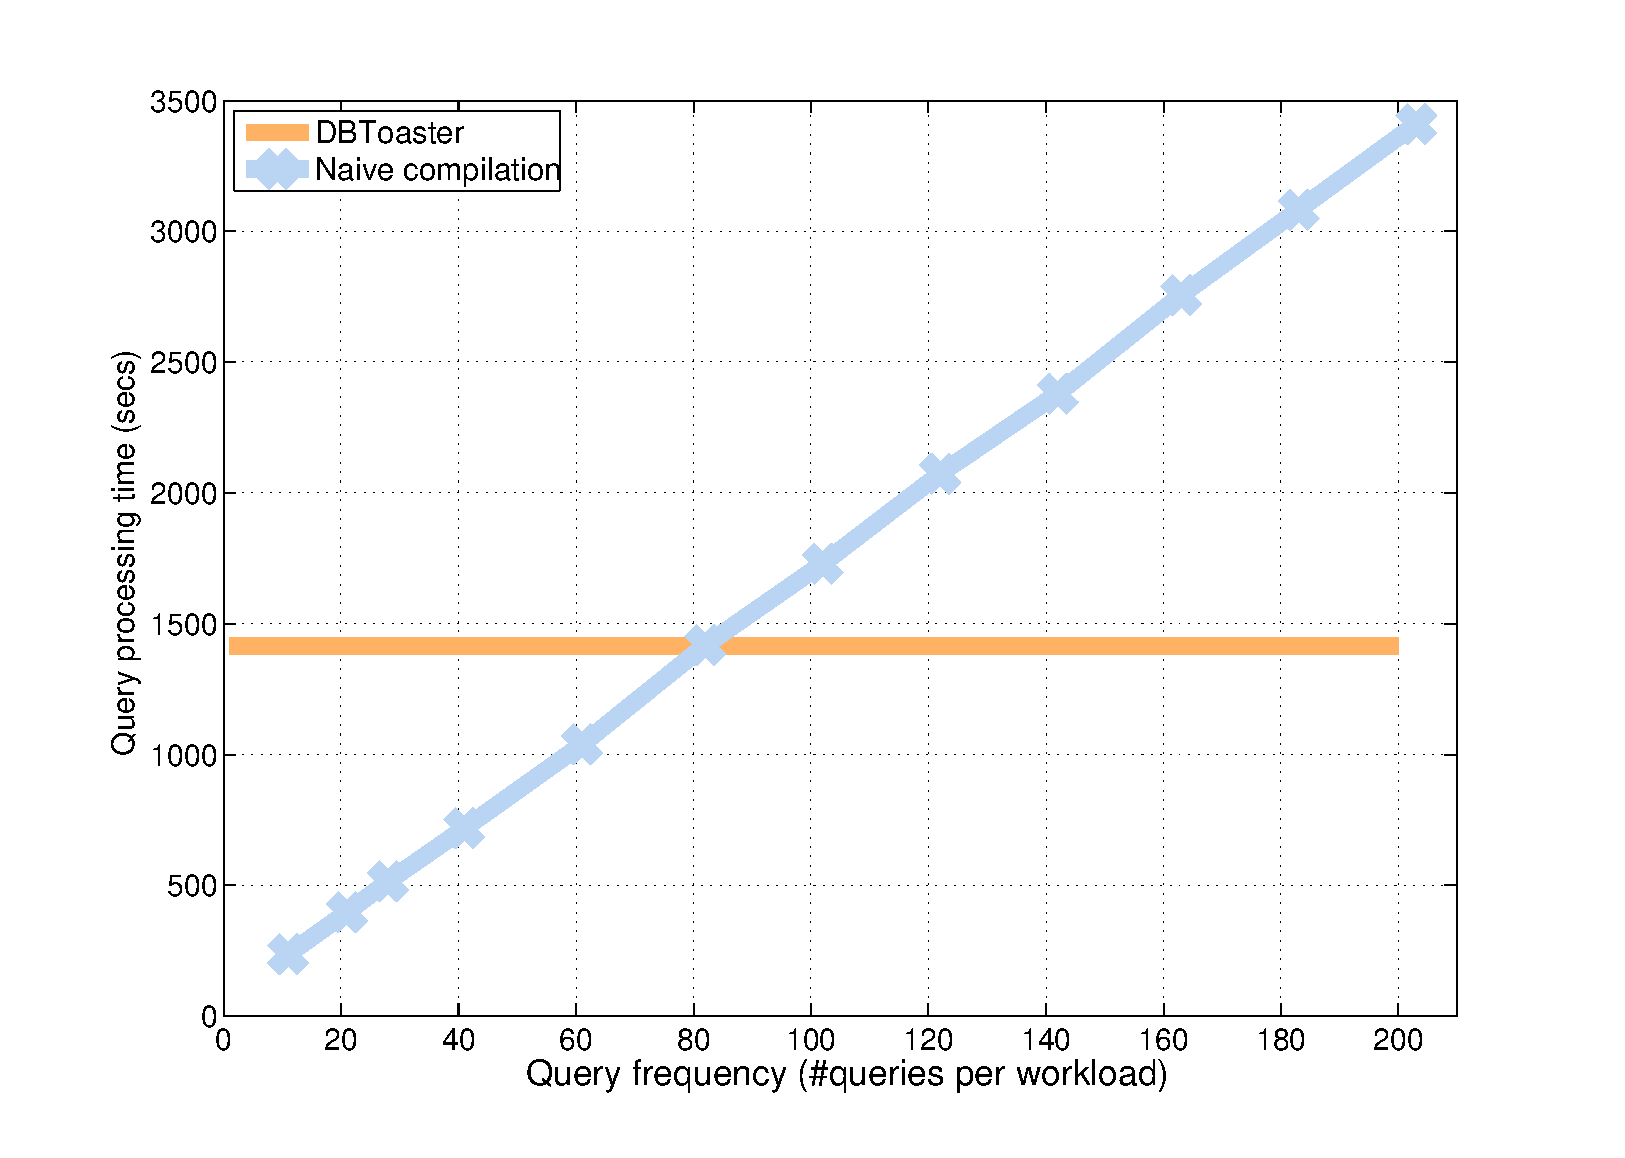
\includegraphics[scale=0.25]{../plots/vwap_query_freq_dn}
\end{center}
\caption{Query frequency limit for VWAP application, indicating the
query execution frequency beyond which DBToaster outperforms the naive query
plan compilation technique.}
\label{fig:vwap_query_freq}
\end{figure}

\begin{figure}
\begin{center}
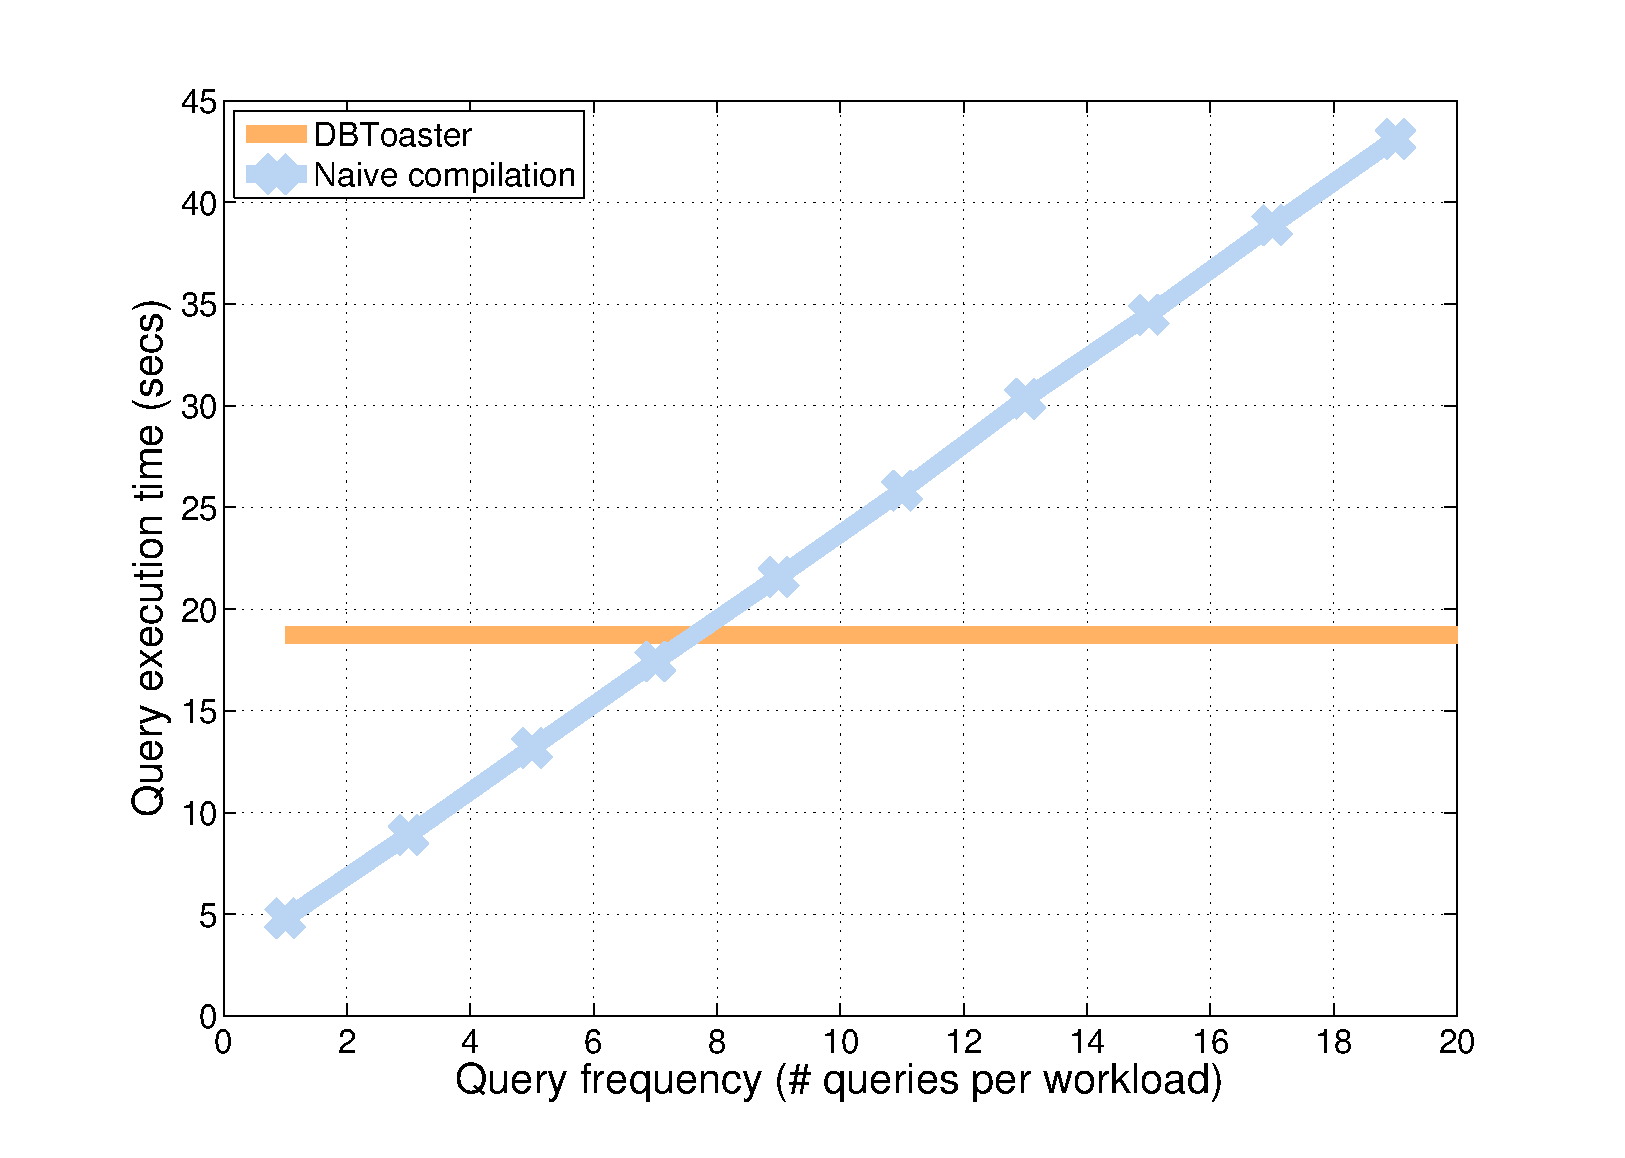
\includegraphics[scale=0.25]{../plots/ssb_query_freq_dn}
\end{center}
\caption{Query frequency limit for warehouse loading application, indicating the
query execution frequency beyond which DBToaster outperforms the naive query
plan compilation technique.}
\label{fig:ssb_query_freq}
\end{figure}

\subsection{Memory Analysis and Batch Execution}


\comment{
Dataset:

\begin{itemize}
  \item TotalView-ITCH dataset: 3 month's worth of MSFT order book messages
  taken from NASDAQ, (~2.2Gb dataset).
  \item Orderbook schema: day, time in us since beginning of day, order id,
  order type, share volume, bid/ask price
\end{itemize}

Queries:

\begin{verbatim}
select * from
  (select ax_bids.mmid, abs(
    sum(ax_bids.volume*
      (act_now.expected_price - ax_bids.price)) -
    sum(ax_asks.volume*
      (ax_asks.price - act_now.expected_price)))
    as ax_bias
  from
    (select mmid, price, volume from bids
       where mmid in axs) as ax_bids,
    (select mmid, price, volume from asks
       where mmid in axs) as ax_asks,
    (select expected_price
        from technical_indicator
        where entrance_condition)
    as act_now
  where ax_bids.mmid = ax_asks.mmid
  group by ax_bids.mmid) as sneaky_ax,
where ax_bias > 10000
\end{verbatim}

Figures:

\begin{enumerate}
  \item Takeaway experiment: end-to-end throughput comparison for a variety of
  insert/update/delete rates. Requires replay speed parameter in data loader.
  Comparison points include Postgres, naive compilation, simple version
  of \compiler, \compiler\ with lazy evaluation, \compiler\ with bulk insert
  mode at 2 or 3 different chunk sizes.

  \item Detail experiment: analyse effect of bulk loading operations compared to
  simple compiler, on a variety of queries, e.g. selectivities and keys.
  Dependent variables for plots: cache hit rates for locality analysis,
  throughput to understand pipelining effects. Is there anything lower lever we
  can do for pipelining?

  \item Detail experiment: selectivity experiment, comparing \compiler\ w/ lazy
  eval, and w/ bulk loading (separately) to next best, for a variety of
  join selectivities and keys.

  \item Detail experiment: space vs recomputation analysis, where we vary the
  maps we keep between extremes of maps from simple decomposition, to full base
  tables.

  \item Quality of compiled code, and compiler effect? e.g. speed provided with
  different -O flags?

\end{enumerate}
}
\nop{

\section{Related Work}
\label{sec:relatedwork}


Database compilers \cite{DBLP:conf/pods/Batory88,DBLP:journals/jiis/BatoryT97}.



A large body of previous research has focused on incremental view maintenance
of relational database queries
\cite{roussopoulos-tods:91,griffin-sigmod:95,colby-sigmod:96,yan-vldb:95,kotidis-tods:01,zhou-vldb:07}.
The focus of this work was always on only one level of delta rewriting
and then using classical relational query processing techniques
based on interpreted query plans and heavyweight monolithic query operators
(such as joins).
In general, however, this means
that the rewritten query is still an arbitrarily complex query (in the number
of joins) and the message passing technique employed in Cumulus is not
applicable.

Most of the previous work on incremental view maintenance does not observe or leverage the fact that aggregation in queries can actually make incremental maintenance {\em easier}, rather than harder, because it greatly reduces the amount of data in the result and because numbers have additional algebraic properties that relations do not have and which allow for further decomposition and optimization of queries.
}

\nop{
Column stores \cite{DBLP:journals/tods/Batory79,DBLP:conf/cidr/KerstenM05,DBLP:conf/vldb/StonebrakerMAHHH07}
are a prominent and successful instance of the recent trend
to abandon rather old database technologies and try out new architectural
para\-digms. Column stores have also been shown to be particularly well suited
for OLAP. However, column stores are fundamentally a secondary storage
concept; in main memory, it does not seem to be particularly meaningful to talk of column or row stores. To date, there has also been no work
on incremental view maintenance in column stores.
Indeed, they are notoriously bad at updating (worse than classical row stores).

H-Store is an OLTP system that abandons classical concurrency control and
recovery baggage for very high performance. It is interesting for the
fresh look at things, and for the viewpoint that even OLTP systems should
be much simpler, nimbler systems than classical databases, which is also
part of the vision behind Cumulus. However, H-Store solves a problem very
different from the one addressed by Cumulus.

Recently, a number of startups have taken off with the idea of running
databases -- even classical technology such as Postgres -- in the cloud
(e.g. Greenplum and Aster Data). While several systems aim at OLAP
applications, none of them allows for true online aggregation as Cumulus does,
and none of the systems takes as radical a lightweight, systemsy approach
as Cumulus.
} % end nop



\section{Conclusions}
\label{sec:conclusions}


We have excluded a number of features from the SQL fragment we support.
MAX and MIN aggregates and the DISTINCT keywords can we added without
fundamental problems, needing only moderate extensions of M3; however,
additional data structures are needed to keep actual database relations
and auxiliary relations
around to check e.g.\ whether a new tuple is already in a relation or what the
second-best tuple is when a maximum or minimum value is removed. We
have built a prototype compiler that implements these features, but lacked the
space for treatment.

Aggregates nested inside FROM and particularly WHERE clauses in general
do not admit recursive compilations of deltas: While it is possible to express
deltas for such queries, the deltas are not structurally simpler than the
input query, and in general, recursive compilation does not terminate,
or does not result in query operator-free code.

It may be rightly observed that we only address single-tuple updates
in this paper and that batching and set-at-a-time techniques have often been
very successful in query processing. We freely admit that our current prototype
does not support batching of updates and the experiments do not report on it.
However, we believe that the compilation approach
should remain unchanged -- delta processing with sets of updates does not
result in code as simple as M3, while the
execution of M3 triggers as generated by our current compiler
can easily be batched. We can profit
particularly from batching message content to send fewer messages in the
distributed system. 

Future work will also address dynamic data partitioning and placement,
and using redundant nodes for reducing view maintenance and query processing
latencies and dealing with node failures.


\bibliographystyle{abbrv}
\bibliography{main}


%\newpage


\appendix


\section{Proof of Proposition~\ref{prop:delta-correct}}


\begin{proof}
It is easy to see that our definition is correct in the case of insertions.
For the deletion case, all we need to show is that
\begin{equation}
\Delta_{-R(\vec{t})}(\alpha + \Delta_{+R(\vec{t})} \alpha) = \alpha.
\label{eq:delta2}
\end{equation}


\def\dtp{\Delta_{+}}
\def\dtm{\Delta_{-}}


We use $\dtp$ and $\dtm$ as shortcuts for $\Delta_{+R(\vec{t})}$
and $\Delta_{-R(\vec{t})}$, respectively.
Let $\alpha' = \alpha+\dtp\alpha$ and $\beta' = \beta+\dtp\beta$.
Consider the expression
\[
\overbrace{\color{white}{\alpha\beta +
\color{black}{\overbrace{\color{white}{
(\dtp \alpha)\beta + (\dtp \alpha)(\dtp \beta)
+ \alpha(\dtp \beta)}}^{\dtp (\alpha\beta)}}}}^{\alpha' \beta'}
\color{white}{+ (\dtp \alpha)(\dtp \beta)}
\]

\vspace{-14mm}

\[
\alpha\beta +
\underbrace{(\dtp \alpha)\beta + (\dtp \alpha)(\dtp \beta)}_{
(\dtp \alpha)\beta'}
+ \underbrace{
\alpha(\dtp \beta) + (\dtp \alpha)(\dtp \beta)}_{\alpha'(\dtp \beta)}
\]
Since $\alpha'\beta' = \alpha\beta + \dtp(\alpha\beta)$,
\begin{equation}
\dtp(\alpha\beta) + (\dtp\alpha)(\dtp\beta) =
(\dtp \alpha)\beta' + \alpha'(\dtp \beta).
\label{eq:delta3}
\end{equation}
We can verify by inspection of our definition that
\begin{equation}
\dtm(\alpha'\beta') + (\dtp \alpha)\beta' + \alpha'(\dtp \beta) =
(\dtp\alpha)(\dtp\beta).
\label{eq:delta4}
\end{equation}
Summing up Equations \ref{eq:delta3} and \ref{eq:delta4}, we obtain
\[
\dtp(\alpha\beta) + \dtm(\alpha'\beta') = 0,
\]
which proves Equation~\ref{eq:delta2}.
%\punto
\end{proof}


\section{Further Examples}


\begin{example}[join on non-key columns]\em
\label{ex:nation}
Given an additional supplier relation, we now ask, for each supplier id (sid),
for the number of customers of the same nation.
\begin{verbatim}
SELECT   S.sid, SUM(1)
FROM     Customer C, Supplier S
WHERE    C.nation = S.nation
GROUP BY S.sid;
\end{verbatim}
The compiler produces the following triggers.
\begin{verbatim}
on insert into Customer (cid, nation) {
  (sid: Supplier.sid) q[sid] += qC[sid, nation];
  qS[nation] += 1
}
on insert into Supplier (sid, nation) {
  q[sid] += qS[nation];
  qC[sid, nation] += 1
}
\end{verbatim}
To understand that this pair
(quadruple, if the deletion triggers are taken into account) of
mutually dependent triggers indeed correctly maintains the query result in q,
verify that auxiliary map {\tt qS} maintains the query
\begin{verbatim}
SELECT nation, SUM(1) FROM Customer GROUP BY nation;
\end{verbatim}
and auxiliary map qC maintains query
\begin{verbatim}
SELECT   sid, nation, SUM(1) FROM Supplier
GROUP BY sid, nation;
\end{verbatim}
The statements updating {\tt q} assure that,
whenever a customer (resp., supplier) is inserted, the count of
matching suppliers (resp., customers) is added to {\tt q}.
\punto
\end{example}


\begin{example}[self-join with complex condition]\em
\label{ex:matchmaking}
In this final example, we consider the data\-base of a matchmaking Web site
that matches humans based on personal profiles. Persons are
represented by a relation Person(\underline{id}, prop), where
prop stands for possibly multiple property col\-umns. Let score$(\cdot, \cdot)$
be a function that maps a pair of property tuples to a compatibility score.
The following query computes, for each person in the database, the number of
matches with compatibility score $\ge 0.9$.
\begin{verbatim}
SELECT   P1.id, SUM(1)
FROM     Person P1, Person P2
WHERE    P1.id <> P2.id
AND      0.9 <= score(P1.prop, P2.prop)
GROUP BY P1.id;
\end{verbatim}

Our compilation approach turns this query into the following M3 program,
with map {\tt q[.]} representing the query result and auxiliary
maps {\tt q1[.,.]} and {\tt q2[.,.,.]}.
\begin{verbatim}
on insert into Person (id, prop) {
  q[id] += q1[id, prop];

  (id2: Person.id) q[id2] += q2[id2, id, prop];

  ((id1, prop1): Person)
  q1[id1, prop1] +=
    if id1<>id and 0.9<=score(prop1, prop) then 1
    else 0;

  ((id2, prop2): Person)
  q2[id, id2, prop2] +=
    if id<>id2 and 0.9<=score(prop, prop2) then 1
    else 0
}
\end{verbatim}
Note that whenever we read a value in such a map program, it has to be
the version of the value from before the start of the program. This is 
ensured in this program because we write q1 and q2 in entries 3 and 4 only
after we have read from q1 and q2 in the first two entries.
But note in particular that also the domains
(id2: Person.id), ((id1, prop1): Person), ((id2, prop2): Person)
are the old ones, before the insertion of the current tuple (id, prop).

The program again has the property that for
each map value to be written, only constantly much work has to be done,
and constantly many lookups have to be made.

This program is the conceptually most difficult so far, so let us look at it
in more detail. It is easy to see that entries 3 and 4 of the program
maintain q1 and q2 as the queries
\begin{verbatim}
q1[id, prop] =
SELECT SUM(1) FROM Person P2
WHERE id<>P2.id and 0.9<=score(prop, P2.prop) 

q2[id1, id, prop] =
SELECT SUM(1) FROM Person P1
WHERE P1.id<>id and 0.9<=score(P1.prop, prop)
AND   P1.id=id1 
\end{verbatim}

Now entry 1 of the program sets the q value for the new person, and
entry 2 updates the q values of the persons that were present previously.
For example, suppose score() is 1 on all inputs and assume that, currently,
there are three persons. Then q is two for each id. Now add a fourth person.
Then q1 is three for the new person and q2 is one for each of the old persons.
By default, q is 0 for the new person before the update.
%
\begin{center}
\begin{tabular}{c|c|c|c|c}
   & before    & \multicolumn{3}{c}{after insert} \\
id & q[id]     & q1[id,.] & q2[id,.,.] & q[id] \\
\hline
1  & 2         &          & 1          & 3 \\
2  & 2         &          & 1          & 3 \\
3  & 2         &          & 1          & 3 \\
4  & undef./0  & 3        &            & 3 \\
\end{tabular}
\end{center}
%
After execution of the on-insert trigger, q is three for each of the four
persons.
\punto
\end{example}


\subsection{Delta processing}


\begin{example}\em
Consider the query
\begin{verbatim}
SELECT SUM(r1.A * r2.B) FROM R r1, R r2
WHERE r1.B=r2.A;
\end{verbatim}
over relation $R$ of schema $(A,B)$
whose deltas on insertion/deletion of
$R$-tuples is
$\duv \AggSum(x*z, R(x,y) \land R(y,z))$ =
$\AggSum(x*z, \duv (R(x,y) \land R(y,z)))$
because $\duv (x*z) = 0$. Since
$\duv R(x,y) = (x=u \land y=v)$ and
$\duv R(y,z) = (y=u \land z=v)$,%
%
\begin{multline*}
\AggSum(x*z, \duv (R(x,y) \land R(y,z))) = \\
\AggSum(x*z, ((x=u \land y=v)^\pm \land R(y,z)) \\
\lor\;
 (R(x,y) \land (y=u \land z=v)^\pm) \\
\lor\;
 ((x=u \land y=v)^\pm \land (y=u \land z=v)^\pm)) =
\end{multline*}

\vspace{-6mm}

\begin{eqnarray*}
&\pm& \AggSum(x*z, x=u \land y=v \land R(y,z)) \\
&\pm& \AggSum(x*z, R(x,y) \land y=u \land z=v) \\
&+  & \AggSum(x*z, x=u \land y=v \land y=u \land z=v).
\end{eqnarray*}
Assuming no other bound variables than $u$ and $v$,
this simplifies to
$\pm \AggSum(u*z, R(v,z))
 \pm \AggSum(x*v, (R(x,u))
 +   (\mbox{if }(u=v) \mbox{ then }(u*v)\mbox{ else }0)$.

Now suppose $R$ currently stores $\{\!| (1,1), (1,1) |\!\}$
(i.e., two copies of tuple $(1,1)$; the query has value 4)
and we insert another copy of tuple $(1,1)$.
Then $\Delta_{+R(1,1)} = 2 + 2 + 1 = 5$, which is
correct: the new value of the query is 9. Now if we delete one of the tuples
$(1,1)$,
$\Delta_{-R(1,1)} = -3 -3 +1 = -5$, and we get back to query value 4. 
\punto
\end{example}


\nop{
Note that $u$ and $v$ are bound variables (to be treated like constants).
Thus, for instance,
$\AggSum(u, R(v, v))$ corresponds to SQL
select u from R where R.A=v and R.B=v,
where we assume that the schema of $R$ is $(A,B)$.
} % end nop


\subsection{Compilation}


\begin{example}\em
Consider a simplified TPC-H like schema with relations O(K, R)
and L(K, P). Orders O have an order key K and the currence exchange rate R fixed for this order (for
foreign customers). Line items L have an {\em order} key
K and a price P. We compile the query
\begin{verbatim}
SELECT SUM(L.P * O.R) FROM O, L WHERE O.K = L.K
\end{verbatim}
which asks for the sum total of all LineItem prices weighted by the exchange
rates of their orders.

The corresponding calculus term is
\[
q[] = \AggSum(p*r, O(k, r) \land L(k, p)).
\]
There are no group-by columns, so we compile as Compile($q$, $\emptyset$, $t$).
We first compute the (insertion) delta for $O$,
\[
\Delta_{+O(k_{O}, r_{O})} q =
\AggSum(p*r, k=k_{O} \land r=r_{O} \land L(k, p))
\]
and simplify with bound variables $\{k_{O}, r_{O}\}$ to
\[
\AggSum(p, L(k_{O}, p))*r_{O}
\]
We extract aggregates to get the pair
\[
\big( m_O[k_{O}]*r_{O},
\{ m_O[k_{O}] \mapsto \AggSum(p, L(k_{O}, p)) \} \big)
\]
Thus $\Delta_{+O(k_{O}, r_{O})} q = m_O[k_{O}]*r_{O}$
and we have to incrementally maintain $m_O[k_O]$.
\begin{eqnarray*}
\Delta_{+L(k_{L}, p_{L})} q &=&
   \AggSum(p*r, O(k, r) \land k=k_{L} \land p=_{L}) \\
&=& p_{L} * m_L[k_{L}]
\end{eqnarray*}
with $m_L[k_{L}] = \AggSum(r, O(k_{L}, r))$ to be incrementally maintained.
We run Compile($m_O$, $\{k_{O}\}$, $\AggSum(p, L(k_{O}, p))$)
and Compile($m_L$, $\{k_{L}\}$, $\AggSum(r, O(k_{L}, r))$) and obtain
\begin{eqnarray*}
\Delta_{+O(k_{OO}, r_{OO})} m_O[k_O] &=& 0 \\
\Delta_{+L(k_{OL}, p_{OL})} m_O[k_O] &=& (k_{OL} = k_O) \;?\; p_{OL} \;:\; 0 \\
\Delta_{+O(k_{LO}, r_{LO})} m_L[k_L] &=& (k_{LO} = k_L) \;?\; r_{LO} \;:\; 0 \\
\Delta_{+L(k_{LL}, p_{LL})} m_L[k_L] &=& 0.
\end{eqnarray*}

We have to incrementally maintain the maps $m_O[\cdot]$ and
$m_L[\cdot]$ for all values in the domain of order keys (i.e., all the order
keys present in the database). However, for bound variables
$k_{OL}, p_{OL}$,
\[
\mbox{for each $k_O$ do $m_O[k_O]$ += $(k_{OL} = k_O) \;?\; p_{OL} \;:\; 0$}
\]
simplifies to $m_O[k_{OL}]$ += $p_{OL}$,
and an analogous simplification applies to $m_L[k_L]$ on insert into $O$.

Overall, we obtain the insertion triggers
\begin{verbatim}
on insert into O(kO,  rO ) { q[] += mO[kO]*rO }
on insert into L(kL,  pL ) { q[] += pL*mL[kL] }
on insert into L(kOL, pOL) { mO[kOL] += pOL }
on insert into O(kLO, rLO) { mL[kLO] += rLO }
\end{verbatim}
The deletion triggers are like the insertion triggers with += replaced by -=.
\punto
\end{example}


\subsection{Foreign-key optimization}


\begin{example}
Consider again Example~\ref{ex:ssb}:
\begin{verbatim}
SELECT   P.partcat, D.year, SUM(revenue)
FROM     Date D, Part P, LineOrder L
WHERE    D.datekey=L.datekey
AND      P.partkey=L.partkey
GROUP BY P.partcat, D.year;

+Date(datekey, year):
 (partcat: Part.partcat)
    m[partcat, year] += mD[datekey, partcat];
 (partkey: Part.partkey)
    mP[partkey, year] += mDP[datekey, partkey];
 mPL[datekey, year] += 1

+Part(partkey, partcat):
 (year: Date.year)
     m[partcat, year] += mP[partkey, year];
 (datekey: Date.datekey)
    mD[datekey, partcat] += mDP[datekey, partkey];
 mDL[partkey, partcat] += 1

+LineOrder(datekey, partkey, revenue):
 (partcat: Part.partcat, year: Date.year)
  m[partcat, year] += revenue
    * mPL[datekey, year] * mDL[partkey, partcat];
 (partcat: Part.partcat) mD[datekey, partcat] +=
    revenue * mDL[partkey, partcat];
 (year: Date.year) mP[partkey, year] +=
    revenue * mPL[datekey, year];
 mDP[datekey, partkey] += revenue;


on insert into Date (datekey, year) {
 mPL[datekey, year] += 1
}
on insert into Part (partkey, partcat) {
 mDL[partkey, partcat] += 1
}
on insert into LineOrder
           (datekey, partkey, revenue) {
  (partcat: Part.partcat, year: Date.year)
  m[partcat, year] += revenue
                    * mPL[datekey, year]
                    * mDL[partkey, partcat]
}
\end{verbatim}
\end{example}


%\section{Figures}


\begin{figure}
\begin{center}
\includegraphics[width=3.5in]{images/MessageFlow.pdf}
\caption{Sequence diagram.}
\end{center}
\end{figure}



\begin{figure}
\begin{center}
\textbf{Schema}
\end{center}
\begin{algorithmic}
\STATE \textbf{create table} customers(cid \textit{int}, nation \textit{int}); 
\STATE \textbf{create table} orders(
\STATE \hspace*{0.1in} oid \textit{int}, o\_cid \textit{int}, opriority \textit{int}, spriority \textit{int},
\STATE \hspace*{0.1in}  \textbf{foreign key}(o\_cid) \textbf{references} customers(cid)
\STATE );
\STATE \textbf{create table} lineitems(
\STATE \hspace*{0.1in} l\_oid \textit{int}, lateship \textit{int}, latedelivery \textit{bool}, shipmode \textit{bool},
\STATE \hspace*{0.1in} \textbf{foreign key}(l\_oid) \textbf{references} orders(oid)
\STATE );
\end{algorithmic}
\begin{center}
\textbf{Query}
\end{center}
\begin{algorithmic}
\STATE \textbf{select} count(*),
\STATE \hspace*{0.1in} nation, cid, oid, opriority, spriority, 
\STATE \hspace*{0.1in} lateship, latedelivery, shipmode 
\STATE \textbf{from} customers, orders, lineitems 
\STATE \textbf{where} o\_cid=cid and l\_oid=oid 
\STATE \textbf{group by cube} 
\STATE \hspace*{0.1in} nation, cid, oid, opriority, spriority, 
\STATE \hspace*{0.1in} lateship, latedelivery, shipmode;
\end{algorithmic}
\caption{An example query that constructs a warehouse for analyzing customer behavior with respect to shipping.  Given a table of customers, orders, and lineitems in those orders, the query builds a datacube over the full join of those tables.}
\label{fig:example}  
\end{figure}



\end{document}  
